\documentclass[11pt,a4paper,oneside]{report}

% ---------------------------------------------------------------------------
% Core Packages & Geometry
% ---------------------------------------------------------------------------
\usepackage[utf8]{inputenc}
\usepackage[T1]{fontenc}
\usepackage{geometry}
\geometry{
  a4paper,
  top=28mm,
  bottom=28mm,
  left=30mm,
  right=25mm,
  headheight=15pt
}

\usepackage{amsmath,amssymb}
\usepackage{booktabs}
\usepackage{tabularx}
\usepackage{longtable}
\usepackage{array}
\usepackage{microtype}
\usepackage{fancyhdr}
\usepackage{titlesec}
\usepackage{enumitem}
\usepackage{tikz}
\usetikzlibrary{shapes.geometric,arrows.meta,positioning,calc,fit,backgrounds}

\usepackage{xcolor}
% MedicalTriage Semantic Palette
\definecolor{NavyDark}{HTML}{090F12}
\definecolor{SlateBackground}{HTML}{F8FAFC}
\definecolor{PrimaryTeal}{HTML}{0F6F73}
\definecolor{AccentIce}{HTML}{38D9C8}
\definecolor{BorderGray}{HTML}{D9E3E6}
\definecolor{TextDark}{HTML}{0C171B}
\definecolor{MutedGray}{HTML}{5B6F76}
\definecolor{UrgentRed}{HTML}{DC2626}
\definecolor{PriorityOrange}{HTML}{EA580C}
\definecolor{RoutineGreen}{HTML}{16A34A}
\definecolor{CodeBg}{HTML}{F1F5F9}

\usepackage{listings}
\lstset{
  backgroundcolor=\color{CodeBg},
  basicstyle=\ttfamily\footnotesize\color{TextDark},
  breakatwhitespace=false,
  breaklines=true,
  captionpos=b,
  commentstyle=\color{MutedGray}\itshape,
  keywordstyle=\color{PrimaryTeal}\bfseries,
  stringstyle=\color{PriorityOrange},
  numbers=none,
  tabsize=2,
  frame=single,
  rulecolor=\color{BorderGray},
  showspaces=false,
  showstringspaces=false,
  showtabs=false,
  xleftmargin=10pt,
  xrightmargin=10pt,
  framesep=6pt
}

\usepackage{hyperref}
\hypersetup{
  colorlinks=true,
  linkcolor=PrimaryTeal,
  citecolor=PrimaryTeal,
  urlcolor=PrimaryTeal,
  pdftitle={MedicalTriage: Engineering Design, Deterministic Safety Engine & Clinical Decision Support Report},
  pdfauthor={MedicalTriage Engineering Team},
  pdfsubject={Final Year Software Engineering Capstone Project Report},
  pdfkeywords={Clinical Decision Support, Deterministic Safety Engine, Multimodal Intake, Emergency Triage, Next.js, TypeScript, MongoDB}
}

% ---------------------------------------------------------------------------
% Header & Footer Configuration
% ---------------------------------------------------------------------------
\pagestyle{fancy}
\fancyhf{}
\fancyhead[L]{\small\color{MutedGray}MedicalTriage: Capstone Engineering Report}
\fancyhead[R]{\small\color{MutedGray}\leftmark}
\fancyfoot[C]{\thepage}
\renewcommand{\headrulewidth}{0.4pt}
\renewcommand{\footrulewidth}{0pt}

\fancypagestyle{plain}{
  \fancyhf{}
  \fancyfoot[C]{\thepage}
  \renewcommand{\headrulewidth}{0pt}
}

% ---------------------------------------------------------------------------
% Title Formatting
% ---------------------------------------------------------------------------
\titleformat{\chapter}[display]
  {\normalfont\huge\bfseries\color{PrimaryTeal}}{\chaptertitlename\ \thechapter}{15pt}{\Huge\color{TextDark}}
\titlespacing*{\chapter}{0pt}{10pt}{20pt}

\titleformat{\section}
  {\normalfont\Large\bfseries\color{PrimaryTeal}}{\thesection}{1em}{}
\titleformat{\subsection}
  {\normalfont\large\bfseries\color{TextDark}}{\thesubsection}{1em}{}
\titleformat{\subsubsection}
  {\normalfont\normalsize\bfseries\color{MutedGray}}{\thesubsubsection}{1em}{}

% ---------------------------------------------------------------------------
% Document Body
% ---------------------------------------------------------------------------
\begin{document}

% ===========================================================================
% Title Page
% ===========================================================================
\begin{titlepage}
  \centering
  \vspace*{20mm}
  
  {\Huge \textbf{\color{PrimaryTeal}MedicalTriage}}\\[5mm]
  {\Large \textbf{A Human-in-the-Loop Clinical Triage and Decision Support System for Resource-Constrained Healthcare Environments}}\\[15mm]
  
  \rule{\textwidth}{1.2pt}\\[10mm]
  
  {\LARGE \textbf{FINAL YEAR CAPSTONE SOFTWARE ENGINEERING PROJECT REPORT}}\\[5mm]
  {\large Department of Computer Science and Engineering}\\[15mm]
  
  \begin{minipage}{0.85\textwidth}
    \centering \itshape \color{MutedGray}
    A comprehensive engineering design, multimodal AI ingestion pipeline,
    deterministic 22-rule safety engine, domain-driven modular monolith topology,
    atomic concurrency review locking, and clinical decision support system report.
  \end{minipage}\\[30mm]
  
  \vfill
  
  \rule{\textwidth}{0.4pt}\\[4mm]
  {\small \textbf{Academic Session:} 2025--2026 \quad $\bullet$ \quad \textbf{Project Version:} 2.4.0 (Full-Stack Research \& Evaluation Release)}
\end{titlepage}

% ===========================================================================
% Abstract
% ===========================================================================
\pagenumbering{roman}
\setcounter{page}{2}

\chapter*{Abstract}
\addcontentsline{toc}{chapter}{Abstract}

Emergency departments and primary outpatient clinics in developing regions operate under persistent, severe resource constraints, processing 80 to 200 walk-in patients per shift with critically skewed clinician-to-patient ratios. Patient presentations are inherently multimodal, consisting of verbal complaints in regional languages, handwritten prescription slips, paper diagnostic lab reports, and visible physical disease manifestations. Traditional paper-based triage workflows suffer from severe transcription overhead, queuing delays, and catastrophic undertriage risks.

This report presents the architectural design, formal requirements, implementation, and empirical verification of \textbf{MedicalTriage}, a production-ready, full-stack clinical decision support and triage system. MedicalTriage implements a multimodal ingestion pipeline integrating Sarvam AI Indic speech-to-text across regional Indian languages (Hindi, Bengali, Tamil, Telugu, Marathi, Gujarati) and Google Gemini / Cloud Vision optical character recognition for structured diagnostic report parsing.

To address the stochastic failure modes and hallucination risks of generative machine learning in safety-critical clinical environments, the system establishes a strict architectural boundary: an isolated Large Language Model synthesizes preliminary differential summaries, while an authoritative, hardcoded \textbf{Deterministic Safety Engine} evaluates twenty-two clinical invariants spanning severe hypoxia, hemodynamic shock, hypertensive crisis, acute stroke (BEFAST), status epilepticus, and pediatric fever boundaries. In any arbitration discrepancy, the system mathematically enforces the highest clinical acuity tier, guaranteeing fail-safe non-inferiority.

The platform incorporates a dynamic First-In, First-Out (FIFO) queue with Service Level Agreement (SLA) countdown timers, distributed atomic concurrency review locking via MongoDB, an immutable 17-event append-only audit ledger, and inter-facility transfer protocols. The architecture is validated across 24 automated Vitest test suites comprising 344 unit and integration test cases, achieving 100\% test passage across all deterministic safety rules and zero regressions in clinical state transitions.

\vspace{1em}
\noindent \textbf{Keywords:} Clinical Decision Support System (CDSS), Emergency Triage, Deterministic Safety Engine, Multimodal Ingestion, Speech-to-Text, Optical Character Recognition, Role-Based Access Control, Immutable Audit Ledger, Next.js, TypeScript, Vitest Verification.

\clearpage

% ===========================================================================
% Table of Contents & Lists
% ===========================================================================
\tableofcontents
\clearpage

\listoffigures
\clearpage

\listoftables
\clearpage

\pagenumbering{arabic}
\setcounter{page}{1}

% ===========================================================================
% Chapter 1: Introduction
% ===========================================================================
\chapter{Introduction}

\section{Healthcare Workflow Background \& Primary Care Realities}
Healthcare delivery systems in developing nations and densely populated jurisdictions operate under persistent, severe resource constraints. In public healthcare ecosystems---particularly within Primary Health Centres (PHCs), Community Health Centres (CHCs), Sub-Divisional Hospitals, and Outpatient Departments (OPDs) of major government teaching hospitals---the ratio of healthcare providers to presenting patients is critically skewed. Medical officers and triage nursing staff routinely process between 80 to 200 walk-in patients during a single 6-hour clinical shift.

In this high-throughput clinical environment, the initial patient intake and triage phase is the most vital determinant of clinical outcomes and operational efficiency. Triage, derived from the French verb \textit{trier} (to sort), represents the formal clinical process of rapidly assessing presenting patients, categorizing their clinical acuity, and assigning queue precedence so that individuals with critical, life-threatening conditions receive immediate clinical intervention, while stable cases are scheduled for routine consultation~\cite{etat2016}.

However, the operational reality of public primary care in India and similar developing settings diverges drastically from idealized emergency room triage protocols utilized in advanced Western hospitals, such as the 5-level Emergency Severity Index (ESI)~\cite{esi2020} or the Canadian Triage and Acuity Scale (CTAS)~\cite{ctas1999}. Walk-in patients in rural and peri-urban clinics arrive without prior appointments, digital health records, or standardized referral summaries.

Instead, their clinical presentation consists of fragmented, multimodal artifacts:
\begin{itemize}[leftmargin=20pt]
  \item \textbf{Unstructured Verbal Complaints:} Spoken in regional dialects and vernacular languages (such as Hindi, Odia, Bengali, Tamil, Telugu, Marathi, or Gujarati) rather than standard medical terminology.
  \item \textbf{Handwritten Prescriptions:} Prior medication slips, paper notes from local registered medical practitioners, or legacy discharge summaries with irregular handwriting.
  \item \textbf{Physical Laboratory Reports:} Printed paper diagnostic strips (e.g., Complete Blood Counts, Widal serology tests, electrolyte panels, or glucose strips) carried physically by the patient.
  \item \textbf{Visible Physical Disease Manifestations:} Non-verbal visual presentations including dermatological eruptions, trauma lacerations, burn boundaries, or localized edema.
\end{itemize}

\section{Problem Statement}
Under current manual workflows, the triage nurse or attending medical officer must manually transcribe verbal histories, decipher handwritten documentation, interpret laboratory report values against physiological norms, inspect physical symptoms, and manually synthesize a coherent clinical summary---all within an allotted clinical window of two to three minutes per patient.

This workflow structure suffers from severe systemic vulnerabilities:
\begin{enumerate}[leftmargin=20pt]
  \item \textbf{High Cognitive Load and Triage Fatigue:} Under high patient volume, clinicians experience cognitive exhaustion, leading to diagnostic oversight and transcription errors.
  \item \textbf{Catastrophic Undertriage Risk:} Time-critical, subtle emergency presentations (such as early sepsis, atypical acute myocardial infarction, or pediatric respiratory distress) risk being misclassified into standard outpatient queues, leading to preventable clinical deterioration and mortality.
  \item \textbf{Linguistic Communication Barriers:} Language discordance between healthcare providers and patients speaking regional vernaculars frequently leads to incomplete symptom capture and missed red-flag symptoms.
  \item \textbf{Disjointed Queue Management:} Absence of centralized, real-time acuity tracking results in unmonitored waiting queues where deteriorating patients go unnoticed.
  \item \textbf{Lack of Clinical Auditability:} Paper-based triage records lack immutable timestamps, cryptographic signatures, or standardized documentation, impeding forensic review and quality governance.
\end{enumerate}

\section{Project Motivation}
The primary motivation of the MedicalTriage project is to engineer an accessible, resilient, and safe clinical decision support platform tailored specifically for high-throughput, resource-constrained primary care environments. By leveraging modern speech recognition and computer vision pipelines, the system automates the friction-heavy data ingestion phase, liberating medical personnel to focus on high-touch clinical assessment.

Crucially, the motivation explicitly rejects the unsafe paradigm of replacing human medical officers with autonomous artificial intelligence. Instead, the project is motivated by a \textbf{Human-in-the-Loop (HITL)} architectural philosophy: artificial intelligence is utilized strictly as a non-diagnostic cognitive accelerator to organize, transcribe, and structure information, while a mathematically verifiable, hardcoded \textbf{Deterministic Safety Engine} enforces strict clinical guardrails, ensuring that human medical officers retain absolute, final authority over patient disposition.

\section{Project Aims \& Objectives}
The core aim of MedicalTriage is to deliver a production-ready, full-stack clinical triage and queue management system that dramatically reduces intake time, standardizes documentation, and eliminates preventable undertriage.

To achieve this overarching aim, the following concrete technical and clinical objectives were established:
\begin{enumerate}[leftmargin=20pt]
  \item \textbf{Multimodal Ingestion Pipeline:} Implement a multi-channel data ingestion architecture capable of transcribing spoken clinical complaints across Indic regional languages via Sarvam AI speech models and extracting structured numerical laboratory parameters from uploaded paper reports via Gemini Vision OCR.
  \item \textbf{Dual-Engine Triage Arbitration:} Design an uncompromised architectural separation between stochastic Large Language Model synthesis and a hardcoded, 22-rule Deterministic Safety Engine, mathematically guaranteeing that the assigned review urgency is never lower than the highest triggered safety invariant.
  \item \textbf{Dynamic Queue Governance \& SLA Tracking:} Develop a real-time clinical queue management engine that calculates dynamic Service Level Agreement (SLA) countdowns per acuity tier, implements automated priority escalation for overdue cases, and executes distributed optimistic concurrency locking to prevent multiple doctors from colliding on the same patient chart.
  \item \textbf{Clinician Review Cockpit \& STN Synthesis:} Provide an ergonomic web workspace that aggregates multimodal evidence into an auto-generated Structured Triage Note (STN), enabling human clinicians to verify, edit, override, and finalize clinical encounters.
  \item \textbf{Enterprise Security \& Immutable Audit Ledger:} Enforce 6-role granular Role-Based Access Control (RBAC), JSON Web Token (JWT) stateless authorization, and an append-only 17-event audit ledger to guarantee regulatory compliance and complete non-repudiation.
  \item \textbf{Exhaustive Verification \& Quality Assurance:} Verify all platform capabilities through a comprehensive automated test suite consisting of 24 test suites and 344 unit, integration, and boundary test cases across core safety, queue, and intake services.
\end{enumerate}

\section{Scope of the Project}
The functional scope of MedicalTriage encompasses:
\begin{itemize}[leftmargin=20pt]
  \item Patient registration, digital electronic consent verification, and demographic indexing.
  \item Audio capture, Indic speech-to-text transcription, and automated medical translation into structured English.
  \item Optical Character Recognition (OCR) parameter parsing for diagnostic lab reports and vitals validation.
  \item Automated triage classification across three clinical urgency tiers: \textbf{URGENT} (1-hour SLA, resus/immediate threat), \textbf{PRIORITY} (4-hour SLA, acute/vulnerable), and \textbf{ROUTINE} (24-hour SLA, non-urgent/stable).
  \item Real-time priority queueing, concurrency locking, and inter-facility transfer workflow management.
  \item Complete administrative logging, user account provisioning, and forensic audit trail inspection.
\end{itemize}

\section{Organization of the Report}
The remainder of this report is organized into the following structured chapters:
\begin{itemize}[leftmargin=20pt]
  \item \textbf{Chapter 2:} Surveys clinical triage scales, emergency workflows, and existing digital triage systems.
  \item \textbf{Chapter 3:} Formally defines the 17 functional requirements, non-functional guarantees, and operational constraints.
  \item \textbf{Chapter 4:} Details the high-level layered architecture, modular monolith design, data flow, and sequence flows.
  \item \textbf{Chapter 5:} Analyzes the selection and rationale for each frontend, backend, database, and AI technology.
  \item \textbf{Chapter 6:} Presents the MongoDB document data model, collection schemas, relationships, and indexing strategy.
  \item \textbf{Chapter 7:} Describes the JWT authentication pipeline, bcrypt adaptive password hashing, and the 6-role RBAC matrix.
  \item \textbf{Chapter 8:} Explains the 4-step clinical intake wizard, electronic consent, and physiological vital signs validation.
  \item \textbf{Chapter 9:} Outlines the Sarvam AI Indic STT and Gemini Vision OCR pipelines and the AI-safety isolation boundary.
  \item \textbf{Chapter 10:} Explores the Deterministic Safety Engine, precedence hierarchy, and all 22 hardcoded clinical safety rules.
  \item \textbf{Chapter 11:} Details the human-in-the-loop review cockpit, STN synthesis, SLA countdowns, and referral handovers.
  \item \textbf{Chapter 12:} Evaluates the STRIDE threat model, data-at-rest/in-transit encryption, and the 17-event immutable audit ledger.
  \item \textbf{Chapter 13:} Highlights key architectural implementation modules, concurrency locks, and code structures.
  \item \textbf{Chapter 14:} Documents the 24 automated Vitest test suites, safety rule boundary fuzzing, and FMEA resilience matrix.
  \item \textbf{Chapter 15:} Details the containerized Docker topology, environment configuration, and infrastructure orchestration.
  \item \textbf{Chapter 16:} Discusses the ergonomic Dark Navy + Teal design system, accessibility tokens, and role-tailored portals.
  \item \textbf{Chapter 17:} Acknowledges technical boundaries, clinical assumptions, and the future research roadmap.
  \item \textbf{Chapter 18:} Summarizes the primary engineering contributions and final concluding evaluations.
\end{itemize}

% ===========================================================================
% Chapter 2: Literature Review & Related Work
% ===========================================================================
\chapter{Literature Review \& Related Work}

\section{Evolution of Clinical Triage Systems}
The systematic sorting of patients based on clinical acuity originated in military trauma medicine during the Napoleonic Wars under Baron Dominique Jean Larrey. In civilian emergency medicine, structured triage systems evolved to manage emergency department overcrowding and ensure equitable allocation of scarce resuscitation facilities~\cite{etat2016}.

Modern emergency departments internationally rely on validated clinical acuity classification scales:
\begin{enumerate}[leftmargin=20pt]
  \item \textbf{Emergency Severity Index (ESI):} Developed in the United States, ESI stratifies patients from Level 1 (Resuscitation) to Level 5 (Non-urgent) based on vital sign stability and predicted healthcare resource utilization (e.g., lab tests, intravenous medications, imaging studies)~\cite{esi2020}.
  \item \textbf{Canadian Triage and Acuity Scale (CTAS):} Widely adopted across the Commonwealth, CTAS assigns mandated physician assessment time targets (e.g., Level 1: Immediate; Level 2: $\le$ 15 minutes; Level 3: $\le$ 30 minutes) based on presenting chief complaint lists and physiological modifiers~\cite{ctas1999}.
  \item \textbf{World Health Organization ETAT:} The Emergency Triage Assessment and Treatment (ETAT) guidelines prioritize pediatric and general presentations into Emergency, Priority, and Non-urgent categories in low-resource environments~\cite{etat2016}.
\end{enumerate}

\section{Analysis of Existing Digital Triage Solutions}
In recent years, several digital healthcare platforms and commercial symptom checkers have emerged attempting to digitize or automate patient triage. Table~\ref{tab:lit_comparison} provides a comparative evaluation of prevalent digital triage approaches against the operational realities of resource-constrained primary care.

\begin{table}[htbp]
  \centering
  \small
  \caption{Comparative Analysis of Clinical Triage Systems and Digital Solutions}
  \label{tab:lit_comparison}
  \begin{tabularx}{\textwidth}{p{2.6cm}p{2.6cm}p{2.8cm}X}
    \toprule
    \textbf{System / Scale} & \textbf{Input Modality} & \textbf{Decision Mechanism} & \textbf{Operational Limitations in Low-Resource Care} \\
    \midrule
    Traditional ESI / CTAS & Manual paper or static EHR entry & Clinical nurse judgment based on decision algorithms & High manual transcription burden; severe cognitive fatigue under surge; lack of real-time queue synchronization. \\
    \addlinespace
    Commercial Consumer Chatbots (e.g., Babylon, Ada) & Text questionnaire / Patient symptom selection & Statistical Bayesian models or conversational NLP & Assumes high patient literacy; requires direct patient English text input; lacks lab OCR parsing and hardcoded safety invariants. \\
    \addlinespace
    Proprietary Hospital EHR Triage (e.g., Epic ASAP) & Structured keyboard entry by triage nurse & Embedded rule triggers and deterministic warnings & Expensive licensing; heavy hardware footprint; requires extensive broadband and localized EHR configuration. \\
    \addlinespace
    Pure LLM Diagnostic Prototypes & Unstructured free-text prompts & Generative language model (e.g., GPT-4, Med-PaLM) & Stochastic hallucination risk; lack of explainability; susceptibility to catastrophic undertriage of atypical emergencies. \\
    \addlinespace
    \textbf{MedicalTriage (This Work)} & \textbf{Multimodal: Indic Voice STT + Paper Lab OCR + Vitals} & \textbf{Dual-Engine: LLM Summarization + Hardcoded 22-Rule Safety Engine} & \textbf{Designed for primary care; offline fallback capability; zero undertriage guarantee via deterministic safety arbitration.} \\
    \bottomrule
  \end{tabularx}
\end{table}

\section{Identified Engineering \& Research Gaps}
A critical synthesis of clinical literature and existing software implementations reveals three fundamental engineering gaps:
\begin{enumerate}[leftmargin=20pt]
  \item \textbf{The Multimodal Friction Gap:} In low-resource public clinics, patients present physical, paper-based diagnostic reports and speak regional dialects. Existing commercial EHRs require manual data entry by busy nursing staff, adding significant operational latency.
  \item \textbf{The AI Hallucination and Safety Gap:} Academic attempts to apply generative Large Language Models directly to clinical triage suffer from stochastic unpredictability. An LLM may misinterpret critical vital signs (e.g., classifying a heart rate of 145 bpm in severe sepsis as mild tachycardia) and inappropriately downgrade acuity.
  \item \textbf{The Workflow Concurrency Gap:} Most primary care clinics lack dynamic electronic queue synchronization, leading to chart lock collisions where multiple doctors unknowingly review the same patient, or overdue cases languish without automated priority escalation.
\end{enumerate}

\section{The MedicalTriage Proposed Paradigm}
To resolve these documented gaps, MedicalTriage implements a hybrid \textbf{Multimodal Intake + Deterministic Safety Architecture}. By utilizing Sarvam AI Indic STT~\cite{sarvam2024} and Gemini Vision OCR~\cite{gemini2023}, the platform removes transcription friction. By enforcing an uncompromised mathematical safety boundary where all AI outputs are strictly bounded by hardcoded deterministic rules derived from validated medical criteria (Sepsis-3~\cite{singer2016}, Glasgow Coma Scale~\cite{teasdale1974}, and ACEP Chest Pain guidelines~\cite{acep2018}), MedicalTriage delivers speed without compromising clinical safety.

% ===========================================================================
% Chapter 3: Requirement Analysis & Specification
% ===========================================================================
\chapter{Requirement Analysis \& Specification}

\section{Stakeholders \& User Personas}
The requirements for MedicalTriage were established through detailed analysis of high-throughput public emergency and outpatient clinical environments. Six distinct user personas interact with the system:
\begin{enumerate}[leftmargin=20pt]
  \item \textbf{Triage Nurse (Intake Specialist):} Responsible for rapid physical intake, capturing electronic patient consent, recording physiological vital signs, initiating multilingual voice recording, and uploading paper lab reports. Needs an ergonomic, high-speed interface with minimal manual typing.
  \item \textbf{Attending Medical Officer (Reviewer):} Responsible for clinical evaluation, reviewing the AI-synthesized differential summary, validating deterministic safety rule flags, performing manual acuity adjustments, and cryptographically finalizing the Structured Triage Note (STN).
  \item \textbf{Triage Supervisor (Charge Physician):} Monitors real-time facility-wide queue health, SLA breach countdowns, bed occupancy, and authorizes inter-facility transfer requests.
  \item \textbf{Facility Administrator:} Manages staff account provisioning, facility directory configurations, and system health monitoring.
  \item \textbf{Forensic Auditor / Legal Compliance Officer:} Conducts post-incident quality audits, inspecting immutable, cryptographically hashed audit trails for forensic non-repudiation.
  \item \textbf{Patient \& Attendant:} The presenting individual requiring clinical care, represented through verified electronic consent and transparent triage queue visibility.
\end{enumerate}

\section{Detailed Functional Requirements (FR-01 to FR-17)}

\subsection{FR-01: User Authentication \& Session Management}
\textbf{Purpose:} Ensure that all clinical actions and data access are attributed to authenticated, accredited healthcare personnel.\\
\textbf{Workflow:} Staff member supplies verified credentials (email/phone and password) over TLS. The server validates bcrypt password hashes and issues a signed JSON Web Token (JWT) with an encoded role claim.\\
\textbf{Inputs:} Authenticated credentials, MFA token (optional).\\
\textbf{Outputs:} Signed JWT access token with 15-minute expiration, user profile payload.\\
\textbf{Security:} Stateless token verification, brute-force rate limiting, SHA-256 session logging.

\subsection{FR-02: Electronic Patient Consent Verification}
\textbf{Purpose:} Mandate explicit patient or guardian consent prior to capturing audio, photographic diagnostic scans, or personal demographics.\\
\textbf{Workflow:} The triage nurse presents the digital consent dialog. The patient or legal guardian acknowledges consent via digital signature or recorded verbal confirmation.\\
\textbf{Inputs:} Patient/guardian consent affirmation, language preference, timestamp.\\
\textbf{Outputs:} Immutable consent boolean flag and ISO-8601 consent timestamp embedded in the encounter.\\
\textbf{Security:} Mandatory pre-condition; intake endpoints reject submissions lacking verified consent.

\subsection{FR-03: Multilingual Speech-to-Text Transcription}
\textbf{Purpose:} Eliminate linguistic barriers and transcription latency during patient intake.\\
\textbf{Workflow:} The triage nurse records presenting chief complaints in regional vernaculars. The audio stream is ingested via Sarvam AI, transcribed into native script, and automatically translated into standardized medical English.\\
\textbf{Inputs:} Raw audio stream (WAV/MP3/WebM), spoken in Hindi, Bengali, Tamil, Telugu, Marathi, or Gujarati.\\
\textbf{Outputs:} Dual-pane transcript: verbatim native script and normalized medical English summary.\\
\textbf{Security:} Server-side streaming over TLS; audio files stored with AES-256 encryption.

\subsection{FR-04: Optical Character Recognition (OCR) Diagnostic Parsing}
\textbf{Purpose:} Digitize physical laboratory test strips and paper diagnostic reports carried by patients.\\
\textbf{Workflow:} Nursing staff capture a photograph or PDF scan of the laboratory report. Gemini Vision OCR extracts text, detects bounding boxes, and parses numerical analyte parameters (e.g., Platelets, WBC, Hemoglobin, Creatinine).\\
\textbf{Inputs:} High-resolution image scan (JPEG/PNG/PDF) $\le$ 10 MB.\\
\textbf{Outputs:} Structured key-value JSON array of laboratory analytes with flagged panic thresholds.\\
\textbf{Security:} Ephemeral pre-signed URLs; automated stripping of non-clinical demographic EXIF data.

\subsection{FR-05: Physiological Vital Signs Validation}
\textbf{Purpose:} Ingest and validate baseline physiological parameters, cross-referencing values against pediatric and adult physiological boundaries.\\
\textbf{Workflow:} Nurse inputs Heart Rate, Blood Pressure, Respiratory Rate, $\text{SpO}_2$, Temperature, Glasgow Coma Scale (GCS), and Numeric Pain Scale. The system validates entries against physiological limits.\\
\textbf{Inputs:} Structured vital signs object.\\
\textbf{Outputs:} Validated vital dataset with computed Mean Arterial Pressure (MAP) and pediatric percentile alerts.\\
\textbf{Security:} Server-side boundary validation rejecting impossible values (e.g., $\text{SpO}_2 > 100\%$).

\subsection{FR-06: AI-Assisted Clinical Triage Inference}
\textbf{Purpose:} Synthesize multimodal intake inputs into a preliminary differential triage assessment.\\
\textbf{Workflow:} Normalized symptoms, translated transcripts, lab analytes, and vitals are structured into an isolated prompt for Gemini. The LLM generates a preliminary acuity tier and clinical summary.\\
\textbf{Inputs:} Structured clinical context JSON.\\
\textbf{Outputs:} Preliminary acuity recommendation (\texttt{URGENT}, \texttt{PRIORITY}, \texttt{ROUTINE}) and differential summary.\\
\textbf{Security:} Isolated context boundary; model outputs treated strictly as advisory drafts.

\subsection{FR-07: Deterministic Safety Engine Rule Evaluation}
\textbf{Purpose:} Enforce hardcoded clinical safety invariants and prevent catastrophic AI undertriage.\\
\textbf{Workflow:} The engine evaluates 22 hardcoded deterministic rules across vitals, lab panic values, and red-flag symptoms. If a rule triggers, the encounter is mathematically locked to at least the rule's minimum safe tier.\\
\textbf{Inputs:} Validated vitals, lab values, and symptom flags.\\
\textbf{Outputs:} Array of triggered rule codes, evaluated minimum safe tier, and arbitration explanation.\\
\textbf{Security:} Pure, auditable deterministic TypeScript logic with 100\% test coverage.

\subsection{FR-08: Dynamic Priority Queue \& SLA Management}
\textbf{Purpose:} Maintain a real-time, acuity-sorted clinical queue with dynamic SLA countdown timers.\\
\textbf{Workflow:} Encounters are queued via FIFO within acuity tiers. Background workers calculate elapsed time against SLA thresholds (\texttt{URGENT}: 1 Hour / 60 min; \texttt{PRIORITY}: 4 Hours / 240 min; \texttt{ROUTINE}: 24 Hours / 1440 min; with 25\% due-soon warning threshold). Overdue cases trigger visual alert pulses.\\
\textbf{Inputs:} Active encounter timestamps and assigned acuity tiers.\\
\textbf{Outputs:} Acuity-sorted queue stream with real-time countdown seconds and overdue breach flags.\\
\textbf{Security:} Sub-second query indexing; optimistic lock state synchronization.

\subsection{FR-09: Atomic Concurrency Review Locking}
\textbf{Purpose:} Prevent multiple physicians from concurrently reviewing and modifying the same patient chart.\\
\textbf{Workflow:} When a medical officer opens an encounter, the platform acquires an atomic database lock via \texttt{Case.findOneAndUpdate}. Other clinicians view the chart in read-only mode with the locking doctor's identity displayed. The lock expires automatically or can be explicitly released.\\
\textbf{Inputs:} Doctor ID, case ID, lock request timestamp.\\
\textbf{Outputs:} Lock acquisition success flag, assigned reviewer binding.\\
\textbf{Security:} MongoDB atomic \texttt{findOneAndUpdate} with conditional lease ownership check.

\subsection{FR-10: Clinician Acuity Override \& Rationale Auditing}
\textbf{Purpose:} Enable human physicians to override system-recommended triage tiers with mandatory accountability.\\
\textbf{Workflow:} A reviewing doctor may adjust the acuity tier. If the adjustment differs from the Safety Engine recommendation, the platform mandates entry of structured clinical rationale text before saving.\\
\textbf{Inputs:} New acuity tier, mandatory text rationale, doctor ID.\\
\textbf{Outputs:} Updated encounter tier, permanent override audit document in the audit ledger.\\
\textbf{Security:} Immutable logging; override justifications cannot be edited or deleted.

\subsection{FR-11: Structured Triage Note (STN) Synthesis \& Finalization}
\textbf{Purpose:} Standardize medical documentation and generate an exportable clinical note.\\
\textbf{Workflow:} The system synthesizes chief complaints, translated narratives, validated vitals, lab tables, safety triggers, and doctor notes into an STN artifact. The doctor verifies and finalizes the document.\\
\textbf{Inputs:} Finalized clinical review parameters, reviewer signature.\\
\textbf{Outputs:} Signed STN JSON payload and exportable clinical summary.\\
\textbf{Security:} Immutability flag and cryptographic audit logging over finalized note payload.

\subsection{FR-12: Inter-Facility Referral Workflow Management}
\textbf{Purpose:} Coordinate patient transfers when the local facility reaches capacity or lacks specialty services.\\
\textbf{Workflow:} The doctor initiates an outbound referral, selecting clinical specialty and transport urgency. Candidate receiving hospitals are queried for real-time bed capacity. Upon acceptance, clinical dossiers transfer securely.\\
\textbf{Inputs:} Target facility ID, transfer urgency, clinical summary dossier.\\
\textbf{Outputs:} Referral state machine transition: \texttt{INITIATED} $\to$ \texttt{ACCEPTED} $\to$ \texttt{EN\_ROUTE} $\to$ \texttt{COMPLETED}.\\
\textbf{Security:} Cross-facility facility-isolation checks and receiving clinician digital custody acknowledgment.

\subsection{FR-13: Bed Availability Handshake Protocol}
\textbf{Purpose:} Ensure receiving facilities formally acknowledge and reserve monitored beds prior to patient transit.\\
\textbf{Workflow:} When a transfer request transitions to \texttt{ACCEPTED}, an atomic reservation is established on the target facility with timeout tracking.\\
\textbf{Inputs:} Receiving facility bed identifier, transfer acceptance token.\\
\textbf{Outputs:} Confirmed bed reservation lock.\\
\textbf{Security:} Automated timeout release if patient dispatch confirmation is not received within SLA.

\subsection{FR-14: Immutable Append-Only Audit Ledger}
\textbf{Purpose:} Record every clinical action, automated assessment, and system modification for forensic non-repudiation.\\
\textbf{Workflow:} Every state-altering API call emits an asynchronous audit event into MongoDB, capturing actor ID, timestamp, action type, prior state, new state, client IP, and metadata hash.\\
\textbf{Inputs:} System events across 17 distinct tracked event types.\\
\textbf{Outputs:} Immutable audit record in \texttt{auditlogs} collection.\\
\textbf{Security:} Database-level and application-level prohibition of UPDATE and DELETE operations.

\subsection{FR-15: Role-Based Access Control (RBAC) Enforcement}
\textbf{Purpose:} Restrict API execution and UI view rendering strictly based on authenticated staff roles.\\
\textbf{Workflow:} Express.js middleware intercepts requests, extracts JWT claims, and validates user roles against the route's required permission matrix.\\
\textbf{Inputs:} Incoming HTTP request with Bearer JWT header.\\
\textbf{Outputs:} Request authorization or HTTP 403 Forbidden rejection.\\
\textbf{Security:} Granular role checks across 6 roles: \texttt{PATIENT}, \texttt{NURSE}, \texttt{HEALTH\_WORKER}, \texttt{DOCTOR}, \texttt{MEDICAL\_OFFICER}, \texttt{ADMIN}.

\subsection{FR-16: Tiered Clinical Data Retention \& Archival}
\textbf{Purpose:} Comply with medical records retention mandates while optimizing persistent storage performance.\\
\textbf{Workflow:} Data moves through four lifecycle retention classes: \texttt{CLINICAL\_CASE}, \texttt{MEDIA\_BLOB}, \texttt{AI\_DERIVED}, and \texttt{AUDIT\_LOG}.\\
\textbf{Inputs:} Encounter age timestamps, retention policies.\\
\textbf{Outputs:} Automated data migration and diagnostic media purging logs.\\
\textbf{Security:} Strict PII minimization prohibiting collection of national identity numbers (Aadhaar/PAN).

\subsection{FR-17: Resilient Offline Fallback Mode}
\textbf{Purpose:} Maintain clinical triage operations during external cloud API or telecommunication outages.\\
\textbf{Workflow:} If cloud AI services (Gemini, Sarvam AI) time out, the system gracefully falls back to local deterministic parsing and prompts staff for manual complaint entry without halting intake.\\
\textbf{Inputs:} Circuit breaker failure trigger.\\
\textbf{Outputs:} Local triage workflow execution with ``AI Degraded'' visual indicator.\\
\textbf{Security:} Pure on-premise execution; vital validation and safety engine remain 100\% operational.

\section{Requirements Summary Matrix}
Table~\ref{tab:req_matrix} provides the complete Functional Requirements Summary Matrix.

\begin{table}[htbp]
  \centering
  \small
  \caption{Functional Requirements Summary Matrix (FR-01 to FR-17)}
  \label{tab:req_matrix}
  \begin{tabularx}{\textwidth}{lp{4.2cm}p{2.6cm}p{2.2cm}X}
    \toprule
    \textbf{Req ID} & \textbf{Requirement Name} & \textbf{Primary Actor} & \textbf{Acuity Impact} & \textbf{Verification Method} \\
    \midrule
    FR-01 & User Authentication \& JWT & All Staff & Governance & Unit / Integration Test \\
    FR-02 & Electronic Patient Consent & Triage Nurse & Regulatory & Automated Schema Validation \\
    FR-03 & Multilingual Indic Speech STT & Triage Nurse & Diagnostic Data & Sarvam AI API Integration \\
    FR-04 & Optical Lab Report OCR & Triage Nurse & Diagnostic Data & Gemini Vision Parsing Test \\
    FR-05 & Physiological Vitals Validation & Triage Nurse & Core Acuity & Physiological Boundary Fuzzing \\
    FR-06 & AI-Assisted Triage Synthesis & System Orchestrator & Advisory Draft & Synthetic Case Evaluation \\
    FR-07 & Deterministic Safety Engine & Safety Subsystem & Invariant Lock & 114 Boundary Test Cases (100\%) \\
    FR-08 & Dynamic Queue \& SLA Timers & Reviewer / Supervisor & Prioritization & Real-Time Countdown Test \\
    FR-09 & Concurrency Review Lock & Medical Officer & Data Integrity & Concurrency Race Condition Test \\
    FR-10 & Clinician Override Auditing & Medical Officer & Accountability & Audit Ledger Signature Check \\
    FR-11 & Structured Triage Note (STN) & Medical Officer & Legal Record & STN Compilation \& Finalize Test \\
    FR-12 & Inter-Facility Referral & Doctor / Supervisor & Continuity of Care & State Machine Transition Test \\
    FR-13 & Bed Handshake Protocol & Bed Manager & Resource Alloc. & Timeout Lease Test \\
    FR-14 & Immutable Audit Ledger & Auditor / Admin & Forensic Audit & Append-Only Permission Test \\
    FR-15 & Role-Based Access Control & Security Middleware & Authorization & 56 RBAC Route Matrix Tests \\
    FR-16 & Data Retention Lifecycle & System Admin & Compliance & Archival Batch Simulation \\
    FR-17 & Resilient Offline Fallback & All Clinical Users & Availability & Circuit Breaker Fault Injection \\
    \bottomrule
  \end{tabularx}
\end{table}

\section{Non-Functional Requirements}
Table~\ref{tab:nfr_matrix} specifies the non-functional performance, availability, and security benchmarks enforced across the platform.

\begin{table}[htbp]
  \centering
  \small
  \caption{Non-Functional Requirements and Operational Benchmarks}
  \label{tab:nfr_matrix}
  \begin{tabularx}{\textwidth}{lp{2.8cm}p{3.2cm}X}
    \toprule
    \textbf{Dimension} & \textbf{Target Metric} & \textbf{Measurement Context} & \textbf{Architectural Mitigation} \\
    \midrule
    API Response Latency & $\le 150\text{ ms}$ (p95) & Standard CRUD operations & In-memory indexing, lean Mongoose projections. \\
    AI Inference Latency & $\le 3000\text{ ms}$ & Gemini + Sarvam pipeline & Asynchronous background workers and streaming APIs. \\
    System Availability & 99.9\% uptime & Primary care operating hours & Dockerized multi-worker clustering, offline fallback. \\
    Concurrency Capacity & $\ge 200$ concurrent requests & Peak emergency intake surge & Stateless Express.js application nodes, connection pooling. \\
    Security \& Encryption & TLS 1.3 / AES-256 & Data in transit and at rest & Enforced HTTPS reverse proxy, encrypted database volumes. \\
    Accessibility & WCAG 2.1 AA compliant & High-contrast Dark Navy/Teal & 4.5:1 minimum contrast ratio, keyboard navigability. \\
    \bottomrule
  \end{tabularx}
\end{table}

% ===========================================================================
% Chapter 4: System Design & Architecture
% ===========================================================================
\chapter{System Design \& Architecture}

\section{System Architectural Overview}
MedicalTriage is engineered as a layered, event-driven modular architecture designed to balance rapid client intake, asynchronous AI processing, deterministic safety validation, and clinical human-in-the-loop review. The architecture enforces three fundamental safety contracts:
\begin{enumerate}[leftmargin=20pt]
  \item \textbf{Input Validation Boundary:} No untrusted client input reaches external AI inference models without defensive schema validation and sanitization.
  \item \textbf{AI-to-Safety Isolation Boundary:} No generative AI output can directly set or modify clinical patient priority without passing through the authoritative, hardcoded Deterministic Safety Engine.
  \item \textbf{Human-in-the-Loop Governance Boundary:} No automated system assessment can alter final clinical disposition, discharge, or inter-facility transfer without explicit sign-off from an accredited medical officer.
\end{enumerate}

\section{High-Level Layered Component Decomposition}
Figure~\ref{fig:layered_arch} illustrates the layered decomposition of the MedicalTriage architecture across four primary tiers: Client Presentation, Ingress \& Security, Core Domain Services, and Data Persistence.

\begin{figure}[htbp]
  \centering
  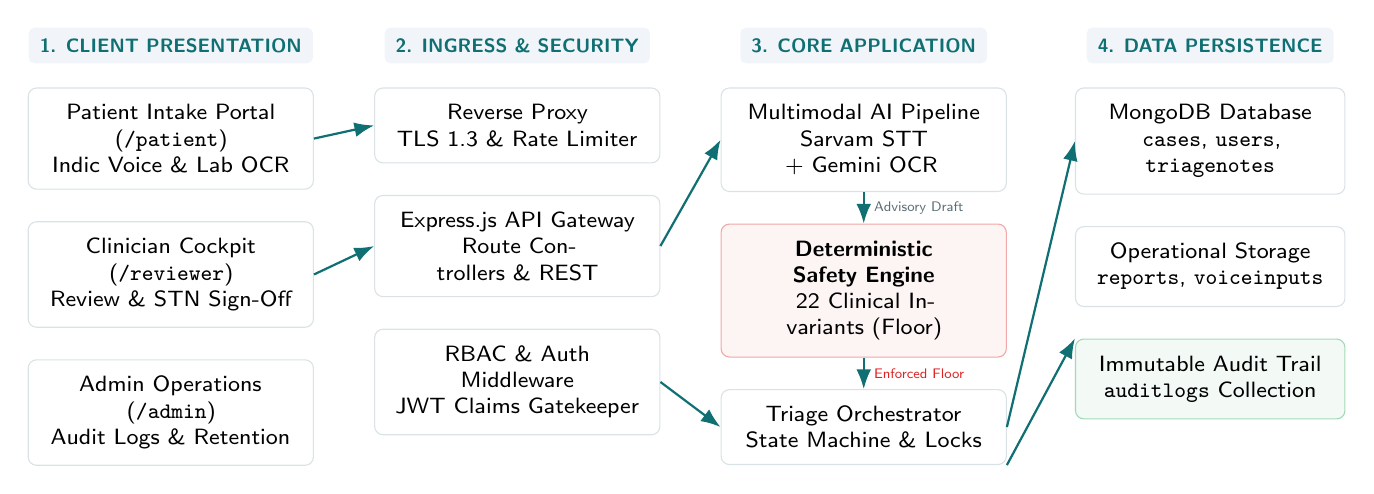
\begin{tikzpicture}[
    box/.style={draw=BorderGray, fill=white, rounded corners=3pt, font=\sffamily\footnotesize, align=center, inner sep=6pt},
    header/.style={font=\sffamily\bfseries\scriptsize, text=PrimaryTeal, fill=CodeBg, rounded corners=2pt, inner sep=4pt},
    arr/.style={-{Latex[length=2.5mm]}, draw=PrimaryTeal, thick}
  ]
    % Column 1: Client Presentation
    \node[header] (t1) at (0, 4) {1. CLIENT PRESENTATION};
    \node[box, below=0.3cm of t1, text width=3.2cm] (c1) {Patient Intake Portal\\(\texttt{/patient})\\Indic Voice \& Lab OCR};
    \node[box, below=0.4cm of c1, text width=3.2cm] (c2) {Clinician Cockpit\\(\texttt{/reviewer})\\Review \& STN Sign-Off};
    \node[box, below=0.4cm of c2, text width=3.2cm] (c3) {Admin Operations\\(\texttt{/admin})\\Audit Logs \& Retention};

    % Column 2: Ingress & Security
    \node[header] (t2) at (4.4, 4) {2. INGRESS \& SECURITY};
    \node[box, below=0.3cm of t2, text width=3.2cm] (i1) {Reverse Proxy\\TLS 1.3 \& Rate Limiter};
    \node[box, below=0.4cm of i1, text width=3.2cm] (i2) {Express.js API Gateway\\Route Controllers \& REST};
    \node[box, below=0.4cm of i2, text width=3.2cm] (i3) {RBAC \& Auth Middleware\\JWT Claims Gatekeeper};

    % Column 3: Core Application
    \node[header] (t3) at (8.8, 4) {3. CORE APPLICATION};
    \node[box, below=0.3cm of t3, text width=3.2cm] (a1) {Multimodal AI Pipeline\\Sarvam STT + Gemini OCR};
    \node[box, below=0.4cm of a1, text width=3.2cm, fill=UrgentRed!5, draw=UrgentRed!40] (a2) {\textbf{Deterministic Safety Engine}\\22 Clinical Invariants (Floor)};
    \node[box, below=0.4cm of a2, text width=3.2cm] (a3) {Triage Orchestrator\\State Machine \& Locks};

    % Column 4: Data Persistence
    \node[header] (t4) at (13.2, 4) {4. DATA PERSISTENCE};
    \node[box, below=0.3cm of t4, text width=3.0cm] (d1) {MongoDB Database\\\texttt{cases}, \texttt{users}, \texttt{triagenotes}};
    \node[box, below=0.4cm of d1, text width=3.0cm] (d2) {Operational Storage\\\texttt{reports}, \texttt{voiceinputs}};
    \node[box, below=0.4cm of d2, text width=3.0cm, fill=RoutineGreen!5, draw=RoutineGreen!40] (d3) {Immutable Audit Trail\\\texttt{auditlogs} Collection};

    % Connectors
    \draw[arr] (c1.east) -- (i1.west);
    \draw[arr] (c2.east) -- (i2.west);
    \draw[arr] (i2.east) -- (a1.west);
    \draw[arr] (a1.south) -- node[right, font=\tiny\sffamily, text=MutedGray] {Advisory Draft} (a2.north);
    \draw[arr] (a2.south) -- node[right, font=\tiny\sffamily, text=UrgentRed] {Enforced Floor} (a3.north);
    \draw[arr] (a3.east) -- (d1.west);
    \draw[arr] (i3.east) -- (a3.west);
    \draw[arr] (a3.south east) -- (d3.north west);

  \end{tikzpicture}
  \caption{MedicalTriage High-Level 4-Tier Layered System Architecture}
  \label{fig:layered_arch}
\end{figure}

\section{Modular Monolith Architectural Justification}
While distributed microservice architectures are popular in large cloud environments, emergency clinical computing introduces constraints where network partitioning, operational latency, and deployment complexity pose existential reliability risks. MedicalTriage adopts a \textbf{Modular Monolith} architecture.

The backend is structured into 24 cohesive domain modules with strict encapsulation boundaries under \texttt{backend/src/modules/}:
\begin{itemize}[leftmargin=20pt]
  \item \textbf{Authentication \& Access Domain:} \texttt{auth}, \texttt{users}.
  \item \textbf{Patient Intake Domain:} \texttt{intake}, \texttt{cases}, \texttt{consent}, \texttt{symptoms}.
  \item \textbf{Multimodal Processing Domain:} \texttt{ai}, \texttt{ocr}, \texttt{reports}, \texttt{vision}, \texttt{voice}, \texttt{translation}.
  \item \textbf{Safety \& Arbitration Domain:} \texttt{safety} (engine, registry, rules, evaluation).
  \item \textbf{Queue \& Concurrency Domain:} \texttt{reviewer}, \texttt{reviews}, \texttt{sla}, \texttt{triage}.
  \item \textbf{Referrals \& Governance Domain:} \texttt{referrals}, \texttt{facilities}, \texttt{notifications}, \texttt{retention}, \texttt{audit}, \texttt{admin}.
\end{itemize}

This design provides single-process in-memory function call performance ($\le 2\text{ ms}$ intra-service latency), eliminates distributed transaction race conditions, and permits frictionless deployment to on-premise hospital local servers.

\section{End-to-End Data Flow \& Case Lifecycle}
Figure~\ref{fig:case_lifecycle} charts the lifecycle of an emergency encounter from physical presentation to clinical resolution.

\begin{figure}[htbp]
  \centering
  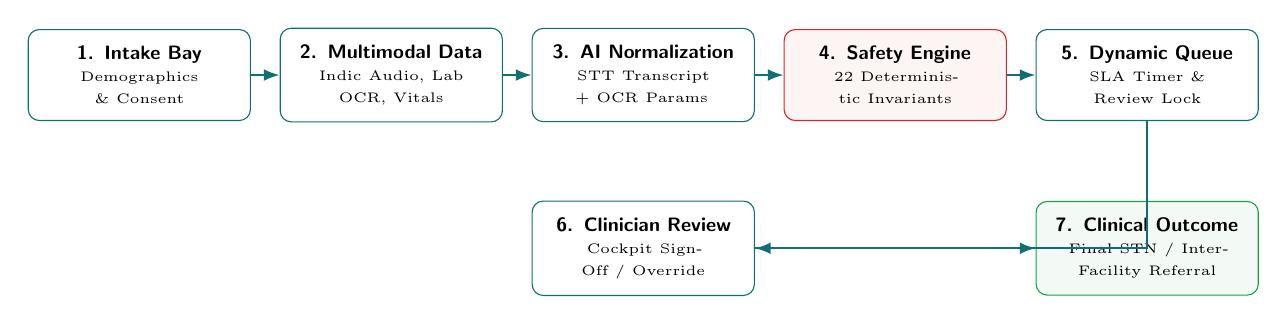
\begin{tikzpicture}[
    stepnode/.style={draw=PrimaryTeal, fill=white, rounded corners=4pt, font=\sffamily\scriptsize\bfseries, align=center, inner sep=6pt, text width=2.4cm},
    arr/.style={-{Latex[length=2mm]}, draw=PrimaryTeal, thick}
  ]
    \node[stepnode] (s1) at (0, 0) {1. Intake Bay\\{\normalfont\tiny Demographics \& Consent}};
    \node[stepnode] (s2) at (3.2, 0) {2. Multimodal Data\\{\normalfont\tiny Indic Audio, Lab OCR, Vitals}};
    \node[stepnode] (s3) at (6.4, 0) {3. AI Normalization\\{\normalfont\tiny STT Transcript + OCR Params}};
    \node[stepnode, draw=UrgentRed, fill=UrgentRed!5] (s4) at (9.6, 0) {4. Safety Engine\\{\normalfont\tiny 22 Deterministic Invariants}};
    \node[stepnode] (s5) at (12.8, 0) {5. Dynamic Queue\\{\normalfont\tiny SLA Timer \& Review Lock}};

    \node[stepnode] (s6) at (6.4, -2.2) {6. Clinician Review\\{\normalfont\tiny Cockpit Sign-Off / Override}};
    \node[stepnode, draw=RoutineGreen, fill=RoutineGreen!5] (s7) at (12.8, -2.2) {7. Clinical Outcome\\{\normalfont\tiny Final STN / Inter-Facility Referral}};

    \draw[arr] (s1) -- (s2);
    \draw[arr] (s2) -- (s3);
    \draw[arr] (s3) -- (s4);
    \draw[arr] (s4) -- (s5);
    \draw[arr] (s5) |- (s6);
    \draw[arr] (s6) -- (s7);
  \end{tikzpicture}
  \caption{End-to-End Patient Triage Lifecycle and State Transitions}
  \label{fig:case_lifecycle}
\end{figure}

\section{Clinical Workflow Sequence Diagrams}
Figures~\ref{fig:seq_auth} to~\ref{fig:seq_review} illustrate the sequence flows across authentication, multimodal intake, and the clinician review workflow.

\begin{figure}[htbp]
  \centering
  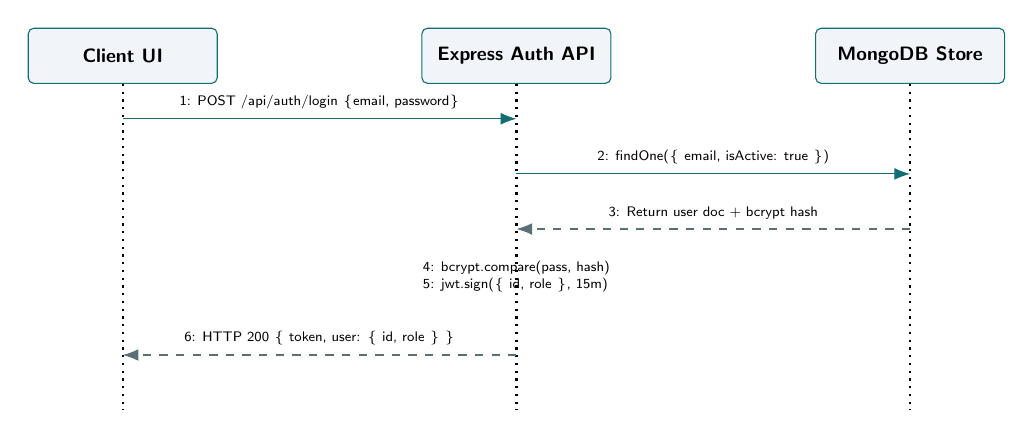
\begin{tikzpicture}[
    actor/.style={draw=PrimaryTeal, fill=CodeBg, rounded corners=2pt, font=\sffamily\scriptsize\bfseries, minimum width=2.4cm, minimum height=0.7cm},
    arr/.style={-{Latex[length=2mm]}, draw=PrimaryTeal},
    ret/.style={-{Latex[length=2mm]}, draw=MutedGray, dashed}
  ]
    \node[actor] (ui) at (0, 0) {Client UI};
    \node[actor] (api) at (5, 0) {Express Auth API};
    \node[actor] (db) at (10, 0) {MongoDB Store};

    \draw[dotted, thick] (ui) -- (0, -4.5);
    \draw[dotted, thick] (api) -- (5, -4.5);
    \draw[dotted, thick] (db) -- (10, -4.5);

    \draw[arr] (0, -0.8) -- node[above, font=\tiny\sffamily] {1: POST /api/auth/login \{email, password\}} (5, -0.8);
    \draw[arr] (5, -1.5) -- node[above, font=\tiny\sffamily] {2: findOne(\{ email, isActive: true \})} (10, -1.5);
    \draw[ret] (10, -2.2) -- node[above, font=\tiny\sffamily] {3: Return user doc + bcrypt hash} (5, -2.2);
    \node[font=\tiny\sffamily, align=left] at (5, -2.8) {4: bcrypt.compare(pass, hash)\\5: jwt.sign(\{ id, role \}, 15m)};
    \draw[ret] (5, -3.8) -- node[above, font=\tiny\sffamily] {6: HTTP 200 \{ token, user: \{ id, role \} \}} (0, -3.8);
  \end{tikzpicture}
  \caption{Sequence Diagram: Authentication and JWT Issuance Protocol}
  \label{fig:seq_auth}
\end{figure}

\begin{figure}[htbp]
  \centering
  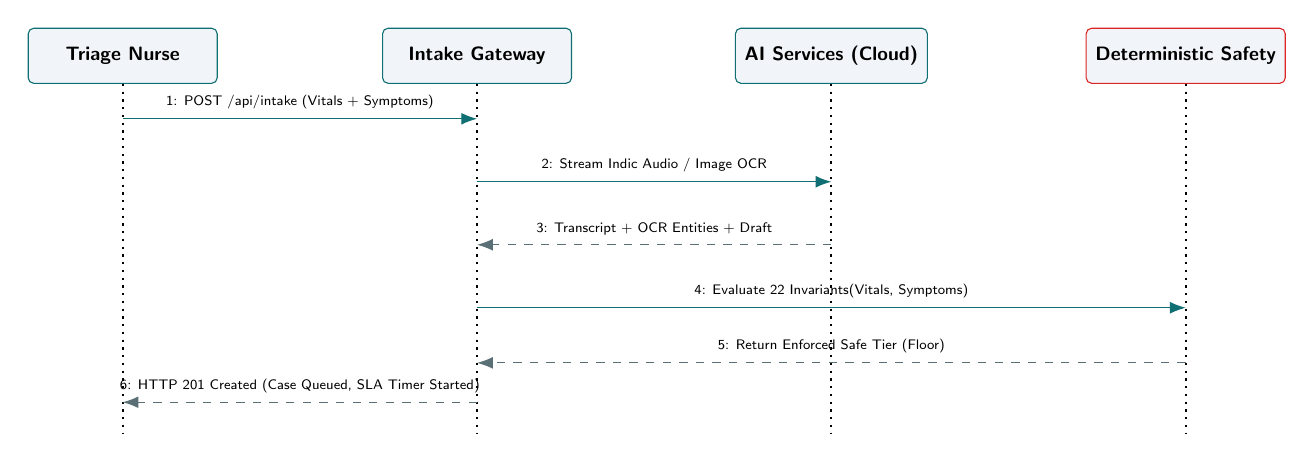
\begin{tikzpicture}[
    actor/.style={draw=PrimaryTeal, fill=CodeBg, rounded corners=2pt, font=\sffamily\scriptsize\bfseries, minimum width=2.4cm, minimum height=0.7cm},
    arr/.style={-{Latex[length=2mm]}, draw=PrimaryTeal},
    ret/.style={-{Latex[length=2mm]}, draw=MutedGray, dashed}
  ]
    \node[actor] (nurse) at (0, 0) {Triage Nurse};
    \node[actor] (gateway) at (4.5, 0) {Intake Gateway};
    \node[actor] (ai) at (9.0, 0) {AI Services (Cloud)};
    \node[actor, draw=UrgentRed] (safety) at (13.5, 0) {Deterministic Safety};

    \draw[dotted, thick] (nurse) -- (0, -4.8);
    \draw[dotted, thick] (gateway) -- (4.5, -4.8);
    \draw[dotted, thick] (ai) -- (9.0, -4.8);
    \draw[dotted, thick] (safety) -- (13.5, -4.8);

    \draw[arr] (0, -0.8) -- node[above, font=\tiny\sffamily] {1: POST /api/intake (Vitals + Symptoms)} (4.5, -0.8);
    \draw[arr] (4.5, -1.6) -- node[above, font=\tiny\sffamily] {2: Stream Indic Audio / Image OCR} (9.0, -1.6);
    \draw[ret] (9.0, -2.4) -- node[above, font=\tiny\sffamily] {3: Transcript + OCR Entities + Draft} (4.5, -2.4);
    \draw[arr] (4.5, -3.2) -- node[above, font=\tiny\sffamily] {4: Evaluate 22 Invariants(Vitals, Symptoms)} (13.5, -3.2);
    \draw[ret] (13.5, -3.9) -- node[above, font=\tiny\sffamily] {5: Return Enforced Safe Tier (Floor)} (4.5, -3.9);
    \draw[ret] (4.5, -4.4) -- node[above, font=\tiny\sffamily] {6: HTTP 201 Created (Case Queued, SLA Timer Started)} (0, -4.4);
  \end{tikzpicture}
  \caption{Sequence Diagram: Multimodal Intake Ingestion and Safety Arbitration Flow}
  \label{fig:seq_intake}
\end{figure}

\begin{figure}[htbp]
  \centering
  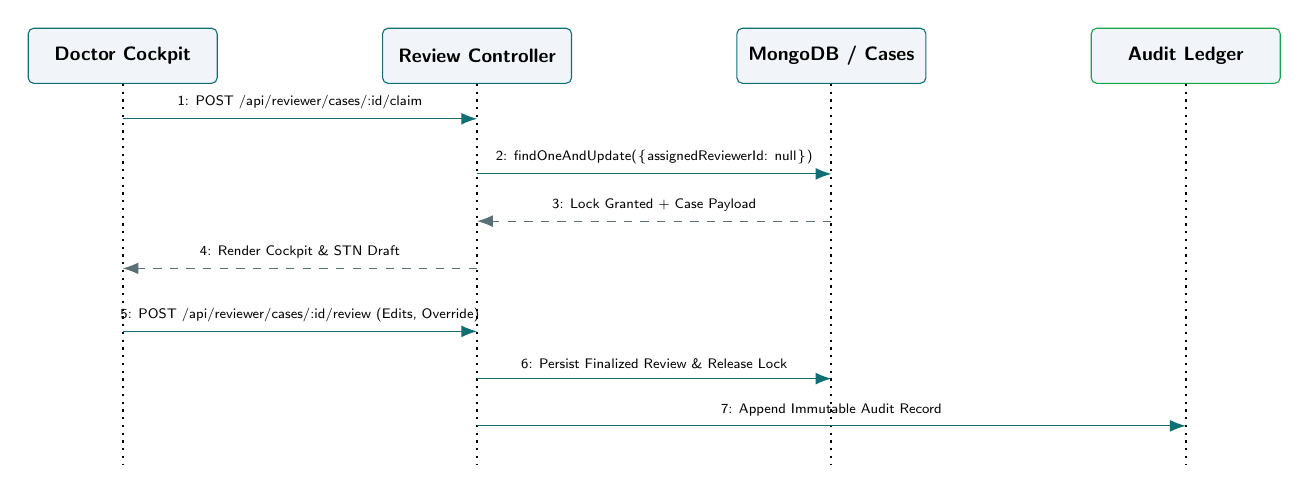
\begin{tikzpicture}[
    actor/.style={draw=PrimaryTeal, fill=CodeBg, rounded corners=2pt, font=\sffamily\scriptsize\bfseries, minimum width=2.4cm, minimum height=0.7cm},
    arr/.style={-{Latex[length=2mm]}, draw=PrimaryTeal},
    ret/.style={-{Latex[length=2mm]}, draw=MutedGray, dashed}
  ]
    \node[actor] (doc) at (0, 0) {Doctor Cockpit};
    \node[actor] (rev) at (4.5, 0) {Review Controller};
    \node[actor] (db) at (9.0, 0) {MongoDB / Cases};
    \node[actor, draw=RoutineGreen] (audit) at (13.5, 0) {Audit Ledger};

    \draw[dotted, thick] (doc) -- (0, -5.2);
    \draw[dotted, thick] (rev) -- (4.5, -5.2);
    \draw[dotted, thick] (db) -- (9.0, -5.2);
    \draw[dotted, thick] (audit) -- (13.5, -5.2);

    \draw[arr] (0, -0.8) -- node[above, font=\tiny\sffamily] {1: POST /api/reviewer/cases/:id/claim} (4.5, -0.8);
    \draw[arr] (4.5, -1.5) -- node[above, font=\tiny\sffamily] {2: findOneAndUpdate(\{assignedReviewerId: null\})} (9.0, -1.5);
    \draw[ret] (9.0, -2.1) -- node[above, font=\tiny\sffamily] {3: Lock Granted + Case Payload} (4.5, -2.1);
    \draw[ret] (4.5, -2.7) -- node[above, font=\tiny\sffamily] {4: Render Cockpit \& STN Draft} (0, -2.7);
    \draw[arr] (0, -3.5) -- node[above, font=\tiny\sffamily] {5: POST /api/reviewer/cases/:id/review (Edits, Override)} (4.5, -3.5);
    \draw[arr] (4.5, -4.1) -- node[above, font=\tiny\sffamily] {6: Persist Finalized Review \& Release Lock} (9.0, -4.1);
    \draw[arr] (4.5, -4.7) -- node[above, font=\tiny\sffamily] {7: Append Immutable Audit Record} (13.5, -4.7);
  \end{tikzpicture}
  \caption{Sequence Diagram: Clinician Review, Concurrency Lock, and STN Sign-Off Flow}
  \label{fig:seq_review}
\end{figure}

% ===========================================================================
% Chapter 5: Technology Stack Selection & Rationale
% ===========================================================================
\chapter{Technology Stack Selection \& Rationale}

\section{Technology Selection Philosophy}
The selection of frameworks, database engines, and runtime dependencies for MedicalTriage was governed by three strict engineering constraints:
\begin{enumerate}[leftmargin=20pt]
  \item \textbf{Low Runtime Latency:} Sub-second responsiveness is mandatory in emergency clinical environments where delays in loading triage queues or vital alarms can impair patient care.
  \item \textbf{High Reliability \& Self-Healing:} Software components must operate without catastrophic crashes, supporting automated circuit breakers and local fallback execution during cloud outages.
  \item \textbf{Maintainability \& Portability:} The entire technology stack must support containerized deployment across both cloud infrastructure and on-premise local server hardware within rural healthcare clinics.
\end{enumerate}

\section{Comparative Technology Analysis}
Table~\ref{tab:tech_stack} provides the comprehensive technology matrix, documenting the selected frameworks, versions, and clinical architectural rationale.

\begin{table}[htbp]
  \centering
  \small
  \caption{MedicalTriage Technology Stack and Architectural Rationale}
  \label{tab:tech_stack}
  \begin{tabularx}{\textwidth}{p{2.6cm}p{3.0cm}p{1.4cm}X}
    \toprule
    \textbf{Layer / Domain} & \textbf{Selected Technology} & \textbf{Version} & \textbf{Engineering Rationale \& Clinical Advantage} \\
    \midrule
    Frontend Framework & Next.js 16 (React 19) & 16.3.x & Server and Client Components; concurrent rendering; high-speed reactive UI state updates; modular component hierarchy for complex triage dashboards. \\
    \addlinespace
    Frontend Styling & Tailwind CSS 4 + Design Tokens & 4.x & Modern CSS styling; design tokens for high-contrast Dark Navy + Deep Teal custom properties; reduced ocular fatigue. \\
    \addlinespace
    Backend Runtime & Node.js / Express & 20.x/22.x & Non-blocking asynchronous I/O event loop; high-concurrency throughput for streaming audio uploads and real-time SLA countdown timers. \\
    \addlinespace
    Backend Language & TypeScript & 5.8.x & End-to-end type safety; strict domain typing across all 24 cohesive backend modules. \\
    \addlinespace
    Primary Database & MongoDB & 7.x & Flexible JSON document model natively matching multimodal medical case trees; atomic document updates for lock management. \\
    \addlinespace
    Speech Recognition & Sarvam AI & API v1 & Lowest Word Error Rate (WER) across Indic vernaculars (Hindi, Bengali, Tamil, Telugu, Marathi, Gujarati); sub-second streaming STT \& translation. \\
    \addlinespace
    Visual OCR \& LLM & Google Gemini 1.5 Pro & API & Native multimodal computer vision for optical lab report parameter extraction; structured JSON schema enforcement. \\
    \addlinespace
    Authentication & JWT + bcrypt & RFC 7519 & Stateless, cryptographically signed bearer tokens; adaptive work factor (12 salt rounds) preventing offline attacks. \\
    \addlinespace
    Automated Testing & Vitest + Supertest & 3.x/7.x & Fast test execution; native ESM support; comprehensive mocking for external cloud APIs across 24 automated test suites (344 tests). \\
    \addlinespace
    Containerization & Docker Compose & v2 & Isolated multi-container deployment orchestrating stateless API nodes, MongoDB clusters, and reverse proxy layers. \\
    \bottomrule
  \end{tabularx}
\end{table}

\section{Database Engine Justification: Document Store vs. Relational}
A critical architectural decision was the selection of a Document Store (MongoDB) over a traditional Relational Database Management System (RDBMS such as PostgreSQL):
\begin{itemize}[leftmargin=20pt]
  \item \textbf{Heterogeneous Multimodal Payloads:} Clinical triage cases contain deeply nested, variable-structure data (e.g., dynamic arrays of OCR bounding boxes, speech transcripts, variable vital sign parameters, and audit entries). In an RDBMS, persisting this requires 8+ normalized join tables, incurring severe query join latency during queue sorting.
  \item \textbf{Atomic Case Encapsulation:} In MongoDB, an entire patient case---including demographic identity, vital signs, audio metadata, safety rule flags, and active concurrency locks---is encapsulated in a single BSON document. Atomic operations (\texttt{\$set}, \texttt{\$push}) execute without multi-table lock contention.
  \item \textbf{Schema Evolution \& Rapid Iteration:} Medical guidelines evolve rapidly. Document collections allow backward-compatible schema expansion without requiring blocking database migration locks.
\end{itemize}

% ===========================================================================
% Chapter 6: Database Design & Data Modeling
% ===========================================================================
\chapter{Database Design \& Data Modeling}

\section{Entity-Relationship Architecture}
The MedicalTriage data architecture is structured around core document collections within MongoDB: \texttt{users}, \texttt{cases}, \texttt{reviews}, \texttt{triagenotes}, \texttt{referrals}, \texttt{auditlogs}, \texttt{symptoms}, \texttt{reports}, \texttt{voiceinputs}, \texttt{visualinputs}, and \texttt{consents}.
Figure~\ref{fig:er_diagram} illustrates the high-level entity relationships, primary keys, and cardinality across primary collections.

\begin{figure}[htbp]
  \centering
  \begin{tikzpicture}[
    entity/.style={draw=BorderGray, fill=white, rounded corners=3pt, font=\sffamily\scriptsize, inner sep=6pt, text width=3.4cm},
    header/.style={font=\sffamily\bfseries\scriptsize, fill=CodeBg, align=center},
    rel/.style={draw=PrimaryTeal, thick, -{Latex[length=2mm]}}
  ]
    \node[entity] (users) at (0, 3) {
      \textbf{USERS (Staff)}\\
      \rule{\linewidth}{0.4pt}
      [PK] \_id: ObjectId\\
      [UQ] email: String\\
      [FLD] passwordHash: String\\
      [FLD] role: UserRole\\
      [FLD] facilityId: String\\
      [FLD] isActive: Boolean
    };

    \node[entity] (cases) at (5.5, 3) {
      \textbf{CASES (Core)}\\
      \rule{\linewidth}{0.4pt}
      [PK] \_id: ObjectId\\
      [UQ] caseNumber: String\\
      [FK] patientId: Ref(users)\\
      [FK] assignedReviewerId: Ref(users)\\
      [FLD] priority: CasePriority\\
      [FLD] status: CaseStatus\\
      [FLD] slaDueAt: Date
    };

    \node[entity] (referrals) at (11, 3) {
      \textbf{REFERRALS (Transit)}\\
      \rule{\linewidth}{0.4pt}
      [PK] \_id: ObjectId\\
      [FK] caseId: Ref(cases)\\
      [FLD] fromFacilityId: String\\
      [FLD] toFacilityId: String\\
      [FLD] status: ReferralStatus
    };

    \node[entity] (reviews) at (2.5, -2) {
      \textbf{REVIEWS (Work)}\\
      \rule{\linewidth}{0.4pt}
      [PK] \_id: ObjectId\\
      [FK] caseId: Ref(cases)\\
      [FK] reviewerId: Ref(users)\\
      [FLD] reviewStatus: String\\
      [FLD] reviewedAt: Date
    };

    \node[entity] (notes) at (8.5, -2) {
      \textbf{TRIAGE NOTES (STN)}\\
      \rule{\linewidth}{0.4pt}
      [PK] \_id: ObjectId\\
      [FK] caseId: Ref(cases)\\
      [FLD] chiefComplaint: String\\
      [FLD] findings: SubDocument\\
      [FLD] safetyFlags: Array\\
      [FLD] isVerified: Boolean
    };

    \draw[rel] (users.east) -- node[above, font=\tiny\sffamily] {1 : N} (cases.west);
    \draw[rel] (cases.east) -- node[above, font=\tiny\sffamily] {1 : N} (referrals.west);
    \draw[rel] (cases.south) -- node[left, font=\tiny\sffamily] {1 : N} (reviews.north);
    \draw[rel] (cases.south) -- node[right, font=\tiny\sffamily] {1 : 1} (notes.north);
  \end{tikzpicture}
  \caption{Entity-Relationship Architecture and Document Schema Dependencies}
  \label{fig:er_diagram}
\end{figure}

\section{Database Collections \& Field Specifications}
Table~\ref{tab:db_collections} summarizes the core collections, key attributes, and data integrity constraints enforced in the MongoDB schema.

\begin{table}[htbp]
  \centering
  \small
  \caption{Primary Database Collections and Schema Attributes}
  \label{tab:db_collections}
  \begin{tabularx}{\textwidth}{lp{2.4cm}p{2.8cm}X}
    \toprule
    \textbf{Collection} & \textbf{Primary Key} & \textbf{Key Foreign References} & \textbf{Core Clinical Attributes \& Invariants} \\
    \midrule
    \texttt{users} & \_id (ObjectId) & None & \texttt{name}, \texttt{email} (unique), \texttt{password} (bcrypt), \texttt{role} (\texttt{PATIENT}, \texttt{NURSE}, \texttt{HEALTH\_WORKER}, \texttt{DOCTOR}, \texttt{MEDICAL\_OFFICER}, \texttt{ADMIN}), \texttt{facilityId}. \\
    \addlinespace
    \texttt{cases} & \_id (ObjectId) & \texttt{patientId} $\to$ \texttt{users}, \texttt{assignedReviewerId} $\to$ \texttt{users} & \texttt{caseNumber} (unique), \texttt{priority} (\texttt{URGENT}, \texttt{PRIORITY}, \texttt{ROUTINE}), \texttt{status} (\texttt{OPEN}, \texttt{IN\_REVIEW}, \texttt{ESCALATED}, \texttt{REFERRED}, \texttt{RESOLVED}, \texttt{CLOSED}), \texttt{slaDueAt}, \texttt{priorityOverride}. \\
    \addlinespace
    \texttt{triagenotes} & \_id (ObjectId) & \texttt{caseId} $\to$ \texttt{cases} & \texttt{chiefComplaint}, \texttt{symptomLog}, \texttt{missingInformation}, \texttt{safetyFlags}, \texttt{isVerified}. \\
    \addlinespace
    \texttt{reviews} & \_id (ObjectId) & \texttt{caseId} $\to$ \texttt{cases}, \texttt{reviewerId} $\to$ \texttt{users} & \texttt{reviewStatus}, \texttt{reviewerNotes}, \texttt{reviewedAt}. \\
    \addlinespace
    \texttt{referrals} & \_id (ObjectId) & \texttt{caseId} $\to$ \texttt{cases} & \texttt{fromFacilityId}, \texttt{toFacilityId}, \texttt{reason}, \texttt{status} (\texttt{PENDING}, \texttt{ACCEPTED}, \texttt{REJECTED}, \texttt{COMPLETED}). \\
    \addlinespace
    \texttt{auditlogs} & \_id (ObjectId) & \texttt{caseId} $\to$ \texttt{cases}, \texttt{actorId} $\to$ \texttt{users} & \texttt{action} (17 event types), \texttt{resourceType}, \texttt{timestamp}, \texttt{outcome}, \texttt{metadata}. \\
    \bottomrule
  \end{tabularx}
\end{table}

\section{Database Indexing \& Performance Optimization}
To ensure sub-150ms query response times during peak emergency triage volume, targeted indexes are established across high-cardinality fields:
\begin{enumerate}[leftmargin=20pt]
  \item \textbf{Queue Sorting Compound Index:} \texttt{\{ status: 1, priority: 1, createdAt: -1 \}}\\
  Enables instant sorting of active patient queues by acuity tier and arrival timestamp (FIFO) without performing in-memory table scans.
  \item \textbf{Facility Scoping Compound Index:} \texttt{\{ facilityId: 1, status: 1 \}}\\
  Enforces multi-tenant facility isolation and high-speed local queue rendering.
  \item \textbf{SLA Alert Compound Index:} \texttt{\{ facilityId: 1, slaDueAt: 1, escalatedAt: 1 \}}\\
  Supports rapid scanning for approaching SLA breaches and automated escalations.
  \item \textbf{User Authentication Unique Index:} \texttt{\{ email: 1 \}, \{ unique: true \}}\\
  Guarantees instant credential lookups during login and enforces user email uniqueness at the storage engine level.
\end{enumerate}

\section{Data Integrity \& Concurrency Guarantees}
In MongoDB, document-level atomicity guarantees that updates to an individual case succeed or fail as an isolated atomic transaction.

When a clinician claims a case from the triage queue, the application executes a conditional atomic update in \texttt{ReviewerService.claimCase}:
\begin{lstlisting}[language=JavaScript]
// Atomic Review Lock Acquisition in MongoDB (ReviewerService.claimCase)
const updatedCase = await Case.findOneAndUpdate(
  { _id: caseId, assignedReviewerId: null, isDeleted: false },
  { $set: { assignedReviewerId: reviewerObjectId } },
  { new: true }
);

if (!updatedCase) {
  const error = new Error('This case was already claimed by another reviewer');
  error.statusCode = 409;
  error.code = 'ASSIGNMENT_CONFLICT';
  throw error;
}
\end{lstlisting}
This query guarantees that if multiple clinicians attempt to claim the same patient case simultaneously, exactly one acquires the lock, while subsequent requests receive an explicit HTTP 409 conflict.

% ===========================================================================
% Chapter 7: Authentication, Authorization & Access Control
% ===========================================================================
\chapter{Authentication, Authorization \& Access Control}

\section{Security Architecture \& Authentication Philosophy}
In healthcare clinical software, authentication and authorization are the foundational security perimeter protecting sensitive Protected Health Information (PHI) and safety-critical clinical triage queues. MedicalTriage enforces stateless, cryptographically signed authentication via JSON Web Tokens (JWT) adhering to RFC 7519 standards.

The access control architecture is designed around the principle of Least Privilege: each user persona is granted only the permissions strictly necessary to execute their defined clinical or administrative responsibilities.

\section{JWT Claims Structure \& bcrypt Password Security}
User passwords are encrypted prior to storage using bcrypt with an adaptive salt work factor of 12 rounds. This computational work factor prevents offline dictionary attacks and rainbow table compromises even in the event of persistent storage exfiltration.

Upon successful credential validation, the authentication service issues an HMAC-SHA256 signed JWT containing a minimal, tamper-evident payload:
\begin{lstlisting}[language=JavaScript]
// JWT Claims Payload Structure
{
  "id": "678f1a2b8e34a1290bc98124",       // User ObjectId
  "email": "doctor@example.com",           // User Email
  "role": "DOCTOR",                        // RBAC Role Claim
  "facilityId": "FAC-DH-CUTTACK",          // Facility Isolation Scope
  "iat": 1728198000,                       // Issued At (Epoch)
  "exp": 1728284400                        // Expiration
}
\end{lstlisting}

\section{Granular 6-Role RBAC Permission Matrix}
MedicalTriage defines six granular roles spanning clinical, emergency, and administrative staff: \texttt{PATIENT}, \texttt{NURSE}, \texttt{HEALTH\_WORKER}, \texttt{DOCTOR}, \texttt{MEDICAL\_OFFICER}, and \texttt{ADMIN}. Table~\ref{tab:rbac_matrix} details the complete permission matrix across all operational modules.

\begin{table}[htbp]
  \centering
  \small
  \caption{Role-Based Access Control (RBAC) Permission Matrix}
  \label{tab:rbac_matrix}
  \begin{tabularx}{\textwidth}{lcccccc}
    \toprule
    \textbf{Operational Capability} & \textbf{PATIENT} & \textbf{NURSE} & \textbf{HLTH\_WRK} & \textbf{DOCTOR} & \textbf{MED\_OFF} & \textbf{ADMIN} \\
    \midrule
    Submit Patient Self-Intake & \checkmark & \checkmark & \checkmark & \checkmark & \checkmark & --- \\
    View Facility Queue & --- & \checkmark & \checkmark & \checkmark & \checkmark & \checkmark \\
    Claim Case Review Lock & --- & \checkmark & \checkmark & \checkmark & \checkmark & --- \\
    Execute AI Extraction & --- & \checkmark & \checkmark & \checkmark & \checkmark & \checkmark \\
    Trigger Safety Engine & --- & \checkmark & \checkmark & \checkmark & \checkmark & \checkmark \\
    Manual Acuity Override & --- & \checkmark & \checkmark & \checkmark & \checkmark & --- \\
    Finalize \& Verify STN Note & --- & \checkmark & \checkmark & \checkmark & \checkmark & --- \\
    Initiate Referral & --- & \checkmark & \checkmark & \checkmark & \checkmark & --- \\
    Acknowledge Inbound Referral & --- & \checkmark & \checkmark & \checkmark & \checkmark & \checkmark \\
    Inspect Immutable Audit Ledger & --- & --- & --- & --- & --- & \checkmark \\
    Admin User Provisioning & --- & --- & --- & --- & --- & \checkmark \\
    Data Retention Purge Trigger & --- & --- & --- & --- & --- & \checkmark \\
    \bottomrule
  \end{tabularx}
\end{table}

\section{Authorization Gatekeeper Middleware Pipeline}
All protected Express.js routes are guarded by a two-stage middleware pipeline:
\begin{enumerate}[leftmargin=20pt]
  \item \textbf{Token Verification Stage (\texttt{authenticateToken}):} Extracts the \texttt{Authorization: Bearer <token>} header, verifies the cryptographic signature, validates that the token has not expired, and attaches the decoded user claims object to \texttt{req.user}.
  \item \textbf{Role Enforcement Stage (\texttt{requireRole([...roles])}):} Inspects \texttt{req.user.role} against the route's allowed role array. If the user's role is not authorized, the middleware immediately halts execution and returns HTTP 403 Forbidden with a structured error message, logging the unauthorized access attempt.
\end{enumerate}

% ===========================================================================
% Chapter 8: Multimodal Patient Intake Pipeline
% ===========================================================================
\chapter{Multimodal Patient Intake Pipeline}

\section{The 4-Step Clinical Intake Wizard}
Patient intake in high-throughput primary care must be rapid, intuitive, and error-resilient. MedicalTriage implements a 4-step linear intake wizard optimized for both touchscreen tablets and desktop workstations:
\begin{enumerate}[leftmargin=20pt]
  \item \textbf{Step 1 --- Demographics \& Electronic Consent:} The intake nurse records patient name, age, biological gender, contact information, and presents the electronic consent dialog. The submission is blocked until explicit digital consent is confirmed.
  \item \textbf{Step 2 --- Multimodal Chief Complaint Ingestion:} The nurse triggers one-tap voice recording in the patient's preferred regional language. The audio stream is uploaded for transcription and translation.
  \item \textbf{Step 3 --- Diagnostic Lab OCR Upload:} Physical paper laboratory slips, test strips, or prior discharge notes are photographed using the device camera. The image is parsed via Gemini Vision OCR, presenting extracted lab values for instant verification.
  \item \textbf{Step 4 --- Physiological Vital Signs Capture:} Baseline vital parameters are entered and validated in real time against physiological limits.
\end{enumerate}

\section{Multimodal Ingestion Pipeline Topology}
Figure~\ref{fig:ingestion_topology} illustrates the multi-channel ingestion architecture and data transformation stages.

\begin{figure}[htbp]
  \centering
  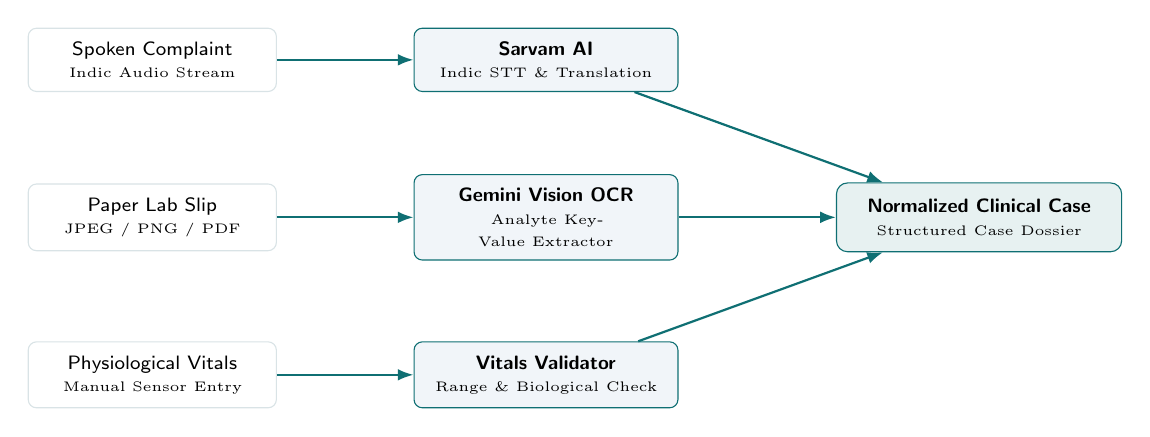
\begin{tikzpicture}[
    inputnode/.style={draw=BorderGray, fill=white, rounded corners=3pt, font=\sffamily\scriptsize, inner sep=5pt, text width=2.8cm, align=center},
    procnode/.style={draw=PrimaryTeal, fill=CodeBg, rounded corners=3pt, font=\sffamily\scriptsize\bfseries, inner sep=5pt, text width=3.0cm, align=center},
    outnode/.style={draw=PrimaryTeal, fill=PrimaryTeal!10, rounded corners=4pt, font=\sffamily\scriptsize\bfseries, inner sep=6pt, text width=3.2cm, align=center},
    arr/.style={-{Latex[length=2mm]}, draw=PrimaryTeal, thick}
  ]
    \node[inputnode] (i1) at (0, 2) {Spoken Complaint\\{\normalfont\tiny Indic Audio Stream}};
    \node[inputnode] (i2) at (0, 0) {Paper Lab Slip\\{\normalfont\tiny JPEG / PNG / PDF}};
    \node[inputnode] (i3) at (0, -2) {Physiological Vitals\\{\normalfont\tiny Manual Sensor Entry}};

    \node[procnode] (p1) at (5, 2) {Sarvam AI\\{\normalfont\tiny Indic STT \& Translation}};
    \node[procnode] (p2) at (5, 0) {Gemini Vision OCR\\{\normalfont\tiny Analyte Key-Value Extractor}};
    \node[procnode] (p3) at (5, -2) {Vitals Validator\\{\normalfont\tiny Range \& Biological Check}};

    \node[outnode] (out) at (10.5, 0) {Normalized Clinical Case\\{\normalfont\tiny Structured Case Dossier}};

    \draw[arr] (i1) -- (p1);
    \draw[arr] (i2) -- (p2);
    \draw[arr] (i3) -- (p3);
    \draw[arr] (p1) -- (out);
    \draw[arr] (p2) -- (out);
    \draw[arr] (p3) -- (out);
  \end{tikzpicture}
  \caption{Multimodal Clinical Intake Ingestion and Normalization Pipeline}
  \label{fig:ingestion_topology}
\end{figure}

\section{Physiological Vital Signs Validation Rules}
The vitals validation engine enforces strict server-side biological boundary checks. Submissions containing impossible parameters (e.g., negative pulse or heart rate $> 300\text{ bpm}$) are rejected with descriptive validation feedback.

Table~\ref{tab:vitals_boundaries} specifies the normal and critical physiological boundary thresholds for adults.

\begin{table}[htbp]
  \centering
  \small
  \caption{Physiological Vital Sign Boundaries and Clinical Validation Limits (Adult)}
  \label{tab:vitals_boundaries}
  \begin{tabularx}{\textwidth}{lp{1.6cm}p{2.2cm}p{2.8cm}X}
    \toprule
    \textbf{Vital Parameter} & \textbf{Unit} & \textbf{Valid Range} & \textbf{Critical Alarm Limits} & \textbf{Clinical Impact} \\
    \midrule
    Heart Rate (HR) & bpm & 20 -- 300 & $< 40$ or $> 140$ & Severe Bradycardia / Tachycardia (Shock risk). \\
    Systolic BP (SBP) & mmHg & 40 -- 280 & $< 80$ or $> 220$ & Severe Hypotension / Hypertensive Crisis. \\
    Diastolic BP (DBP) & mmHg & 20 -- 180 & $> 120$ & Hypertensive Emergency. \\
    Oxygen Saturation ($\text{SpO}_2$) & \% & 50 -- 100 & $< 90\%$ ($< 88\%$ in COPD) & Severe Hypoxemia ($\to$ Immediate Oxygenation). \\
    Respiratory Rate (RR) & bpm & 4 -- 80 & $< 8$ or $> 35$ & Impending Respiratory Failure. \\
    Body Temperature & $^\circ\text{C}$ & 28.0 -- 45.0 & $< 35.0$ or $> 40.5$ & Hypothermia / Hyperpyrexia. \\
    Glasgow Coma Scale & --- & 3 -- 15 & $\le 8$ & Severe Coma / Unprotected Airway. \\
    Pain Score (VAS) & --- & 0 -- 10 & $\ge 8$ & Severe Acute Intractable Pain. \\
    \bottomrule
  \end{tabularx}
\end{table}

% ===========================================================================
% Chapter 9: AI & Multimodal Processing Pipelines
% ===========================================================================
\chapter{AI \& Multimodal Processing Pipelines}

\section{Multilingual Indic Speech Recognition Engine}
A foundational capability of MedicalTriage is the real-time transcription and translation of spoken patient complaints across India's diverse linguistic landscape. The platform integrates Sarvam AI's speech foundation models~\cite{sarvam2024}, optimized for domain-specific clinical vocabulary and accented regional Indic speech.

The speech processing pipeline executes three sequential operations:
\begin{enumerate}[leftmargin=20pt]
  \item \textbf{Acoustic Stream Ingestion:} Audio is captured at a minimum sample rate of 16 kHz in mono PCM/WebM format and streamed over TLS to the backend.
  \item \textbf{Vernacular Transcription:} Sarvam AI's multi-lingual acoustic model transcribes the speech into the patient's native regional script across supported languages: Hindi (\texttt{hi}), Odia (\texttt{or}), Bengali (\texttt{bn}), Tamil (\texttt{ta}), Telugu (\texttt{te}), Marathi (\texttt{mr}), and Gujarati (\texttt{gu}).
  \item \textbf{Clinical Medical Normalization:} The vernacular text is translated into standardized medical English, normalizing colloquial symptom expressions (e.g., translating Gujarati colloquial \textit{"Chhatima bhare daban"} to \textit{"crushing substernal chest pressure"}).
\end{enumerate}

\section{Optical Character Recognition (OCR) for Diagnostic Reports}
Patients presenting to public emergency departments frequently carry physical paper laboratory reports generated by disparate external diagnostic facilities. MedicalTriage leverages Google Gemini 1.5 Pro~\cite{gemini2023} via its native multimodal computer vision API to parse unstructured paper artifacts into structured JSON datasets.

The OCR prompt instructs the vision model to detect report orientation, isolate tabular analyte matrices, extract numerical values and reference ranges, and flag clinical panic values (e.g., Platelet count $< 20,000/\mu\text{L}$ or Serum Potassium $> 6.5\text{ mEq/L}$).

\section{The AI-to-Safety Isolation Boundary}
Figure~\ref{fig:ai_isolation} illustrates the core safety boundary governing AI processing within MedicalTriage.

\begin{figure}[htbp]
  \centering
  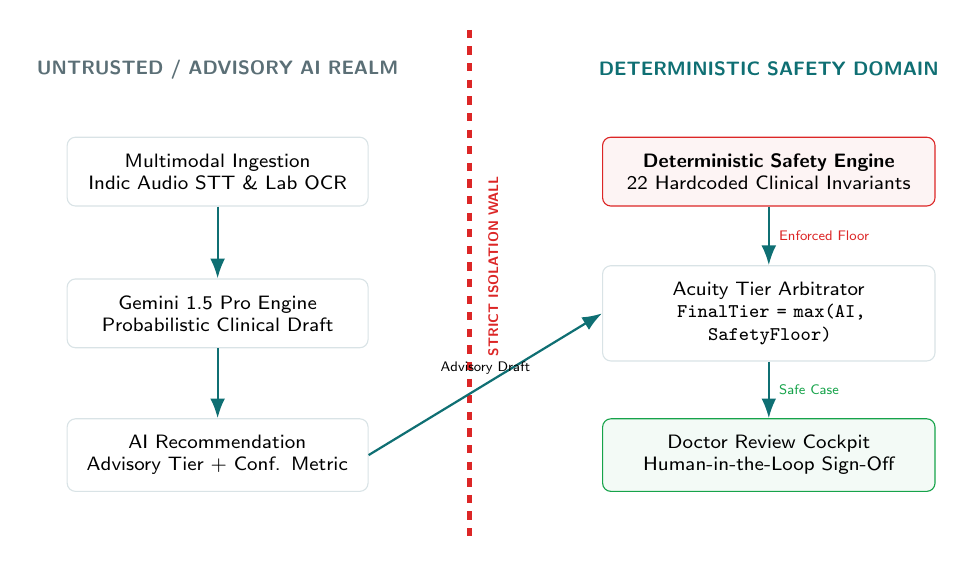
\begin{tikzpicture}[
    box/.style={draw=BorderGray, fill=white, rounded corners=3pt, font=\sffamily\scriptsize, align=center, inner sep=6pt},
    wall/.style={draw=UrgentRed, dashed, ultra thick},
    arr/.style={-{Latex[length=2.5mm]}, draw=PrimaryTeal, thick}
  ]
    % Untrusted Realm
    \node[font=\sffamily\bfseries\scriptsize, text=MutedGray] at (2, 2.5) {UNTRUSTED / ADVISORY AI REALM};
    \node[box, text width=3.4cm] (ai1) at (2, 1.2) {Multimodal Ingestion\\Indic Audio STT \& Lab OCR};
    \node[box, text width=3.4cm] (ai2) at (2, -0.6) {Gemini 1.5 Pro Engine\\Probabilistic Clinical Draft};
    \node[box, text width=3.4cm] (ai3) at (2, -2.4) {AI Recommendation\\Advisory Tier + Conf. Metric};

    % Isolation Wall
    \draw[wall] (5.2, 3) -- (5.2, -3.5);
    \node[font=\sffamily\bfseries\tiny, text=UrgentRed, rotate=90] at (5.5, 0) {STRICT ISOLATION WALL};

    % Deterministic Realm
    \node[font=\sffamily\bfseries\scriptsize, text=PrimaryTeal] at (9, 2.5) {DETERMINISTIC SAFETY DOMAIN};
    \node[box, draw=UrgentRed, fill=UrgentRed!5, text width=3.8cm] (saf1) at (9, 1.2) {\textbf{Deterministic Safety Engine}\\22 Hardcoded Clinical Invariants};
    \node[box, text width=3.8cm] (saf2) at (9, -0.6) {Acuity Tier Arbitrator\\\texttt{FinalTier = max(AI, SafetyFloor)}};
    \node[box, draw=RoutineGreen, fill=RoutineGreen!5, text width=3.8cm] (saf3) at (9, -2.4) {Doctor Review Cockpit\\Human-in-the-Loop Sign-Off};

    \draw[arr] (ai1) -- (ai2);
    \draw[arr] (ai2) -- (ai3);
    \draw[arr] (ai3.east) -- node[above, font=\tiny\sffamily] {Advisory Draft} (saf2.west);
    \draw[arr] (saf1.south) -- node[right, font=\tiny\sffamily, text=UrgentRed] {Enforced Floor} (saf2.north);
    \draw[arr] (saf2.south) -- node[right, font=\tiny\sffamily, text=RoutineGreen] {Safe Case} (saf3.north);
  \end{tikzpicture}
  \caption{Architectural Isolation Boundary Separating Generative AI from the Deterministic Safety Engine}
  \label{fig:ai_isolation}
\end{figure}

The boundary guarantees that:
\begin{itemize}[leftmargin=20pt]
  \item Generative AI models operate purely as \textbf{advisory draft generators} and information summarizers.
  \item The output of the AI pipeline has \textbf{zero direct authority} to downgrade a patient's triage tier below the minimum threshold calculated by the Deterministic Safety Engine.
  \item Processing errors, missing data, or uncertain outputs automatically fail-safe to \texttt{PRIORITY} review.
\end{itemize}

% ===========================================================================
% Chapter 10: The Deterministic 22-Rule Safety Engine
% ===========================================================================
\chapter{The Deterministic 22-Rule Safety Engine}

\section{Clinical Neutrality Contract \& Design Philosophy}
The Deterministic Safety Engine is the core clinical risk-governance subsystem of MedicalTriage. In safety-critical emergency medicine, delegating patient triage priority to probabilistic Large Language Models introduces catastrophic risks of non-deterministic outputs, latent bias, and unexplainable undertriage.

To provide absolute clinical certifiability and algorithmic explainability, MedicalTriage enforces a strict \textbf{Clinical Neutrality Contract}:
\begin{enumerate}[leftmargin=20pt]
  \item \textbf{Non-Diagnostic Mandate:} The Safety Engine does not establish autonomous medical diagnoses or prescribe pharmaceuticals. It assigns an operational workflow review priority (\texttt{URGENT}, \texttt{PRIORITY}, or \texttt{ROUTINE}) to govern clinical queue precedence.
  \item \textbf{AI Priority Isolation:} Large Language Models and generative AI agents are strictly prohibited from assigning or downgrading clinical priority. AI models provide structured draft summaries tagged with \texttt{AI\_GENERATED} provenance badges, while the authoritative Deterministic Safety Engine calculates the case priority.
  \item \textbf{Deterministic Invariance:} Given identical input parameters (vital signs, structured symptoms, laboratory values, and processing confidence states), the Safety Engine is mathematically guaranteed to execute the exact same rule evaluations and return identical priority tiers.
  \item \textbf{Monotonic Safety Hierarchy:} If any clinical invariant or system uncertainty rule is triggered, the platform enforces the highest applicable severity tier:
  \begin{equation}
    \text{Final Priority} = \max(\text{Rule}_1, \text{Rule}_2, \dots, \text{Rule}_{22})
  \end{equation}
  where $\texttt{URGENT} > \texttt{PRIORITY} > \texttt{ROUTINE}$ in ordinal escalation precedence.
\end{enumerate}

\section{Deterministic Decision Tree Flow}
Figure~\ref{fig:decision_tree} depicts the hierarchical evaluation logic executed by the Deterministic Safety Engine for every clinical encounter.

\begin{figure}[htbp]
  \centering
  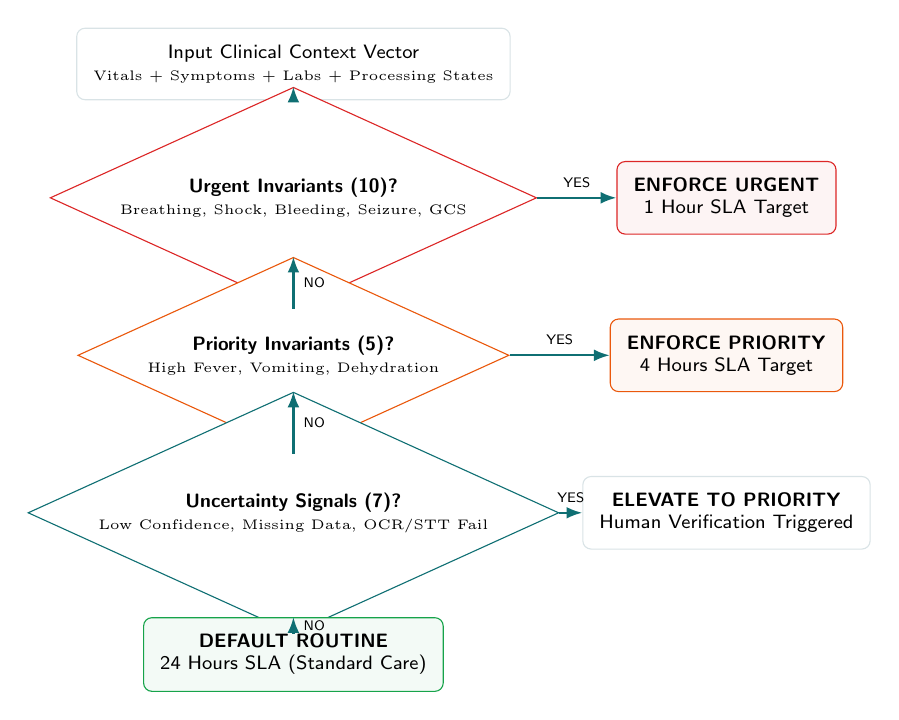
\begin{tikzpicture}[
    decision/.style={diamond, draw=PrimaryTeal, fill=white, aspect=2.2, font=\sffamily\scriptsize\bfseries, align=center, inner sep=3pt},
    action/.style={draw=BorderGray, fill=white, rounded corners=3pt, font=\sffamily\scriptsize, align=center, inner sep=6pt},
    arr/.style={-{Latex[length=2mm]}, draw=PrimaryTeal, thick}
  ]
    \node[action] (in) at (0, 3.5) {Input Clinical Context Vector\\{\normalfont\tiny Vitals + Symptoms + Labs + Processing States}};
    \node[decision, draw=UrgentRed] (d1) at (0, 1.8) {Urgent Invariants (10)?\\{\normalfont\tiny Breathing, Shock, Bleeding, Seizure, GCS}};
    \node[action, draw=UrgentRed, fill=UrgentRed!5] (a1) at (5.5, 1.8) {\textbf{ENFORCE URGENT}\\1 Hour SLA Target};

    \node[decision, draw=PriorityOrange] (d2) at (0, -0.2) {Priority Invariants (5)?\\{\normalfont\tiny High Fever, Vomiting, Dehydration}};
    \node[action, draw=PriorityOrange, fill=PriorityOrange!5] (a2) at (5.5, -0.2) {\textbf{ENFORCE PRIORITY}\\4 Hours SLA Target};

    \node[decision] (d3) at (0, -2.2) {Uncertainty Signals (7)?\\{\normalfont\tiny Low Confidence, Missing Data, OCR/STT Fail}};
    \node[action] (a3) at (5.5, -2.2) {\textbf{ELEVATE TO PRIORITY}\\Human Verification Triggered};

    \node[action, draw=RoutineGreen, fill=RoutineGreen!5] (def) at (0, -4.0) {\textbf{DEFAULT ROUTINE}\\24 Hours SLA (Standard Care)};

    \draw[arr] (in) -- (d1);
    \draw[arr] (d1) -- node[above, font=\tiny\sffamily] {YES} (a1);
    \draw[arr] (d1) -- node[right, font=\tiny\sffamily] {NO} (d2);
    \draw[arr] (d2) -- node[above, font=\tiny\sffamily] {YES} (a2);
    \draw[arr] (d2) -- node[right, font=\tiny\sffamily] {NO} (d3);
    \draw[arr] (d3) -- node[above, font=\tiny\sffamily] {YES} (a3);
    \draw[arr] (d3) -- node[right, font=\tiny\sffamily] {NO} (def);
  \end{tikzpicture}
  \caption{Deterministic Safety Engine Hierarchical Evaluation Decision Tree}
  \label{fig:decision_tree}
\end{figure}

\section{Exhaustive Technical Breakdown of All 22 Deterministic Safety Rules}
The engine evaluates twenty-two clinical safety rules codified within the system's service layer (\texttt{backend/src/modules/safety/safety.registry.ts}), organized into three distinct categories:

\subsection{Category 1: Clinical Urgent Invariant Rules (10 Rules)}

\begin{enumerate}[leftmargin=20pt]
  \item \textbf{URGENT\_HUMAN\_ESCALATION}\\
  \textit{Clinical Criteria:} Explicit manual escalation triggered by an intake triage nurse or reviewing medical officer.\\
  \textit{Enforced Tier:} \texttt{URGENT} (1 Hour SLA).\\
  \textit{Clinical Invariant:} Immediate human clinician authority supersedes all automated baselines.

  \item \textbf{URGENT\_SEVERE\_BREATHING}\\
  \textit{Clinical Criteria:} Acute respiratory distress, stridor, cyanosis, or $\text{SpO}_2 < 90\%$ on ambient air.\\
  \textit{Enforced Tier:} \texttt{URGENT} (1 Hour SLA).\\
  \textit{Clinical Invariant:} Severe hypoxemia causes rapid decompensation requiring immediate oxygenation.

  \item \textbf{URGENT\_CHEST\_PAIN\_BREATHING}\\
  \textit{Clinical Criteria:} Acute substernal crushing chest pain radiating to arm/jaw, accompanied by dyspnea or diaphoresis.\\
  \textit{Enforced Tier:} \texttt{URGENT} (1 Hour SLA).\\
  \textit{Clinical Invariant:} Suspected Acute Coronary Syndrome (ACS / STEMI) requires rapid ECG acquisition.

  \item \textbf{URGENT\_ALTERED\_CONSCIOUSNESS}\\
  \textit{Clinical Criteria:} Unresponsiveness, profound lethargy, confusion, or Glasgow Coma Scale $\le 8$.\\
  \textit{Enforced Tier:} \texttt{URGENT} (1 Hour SLA).\\
  \textit{Clinical Invariant:} Coma and altered mental status indicate acute cerebral compromise or unprotected airway.

  \item \textbf{URGENT\_SEVERE\_BLEEDING}\\
  \textit{Clinical Criteria:} Pulsatile arterial external hemorrhage, massive hematemesis, or melena with hypotension.\\
  \textit{Enforced Tier:} \texttt{URGENT} (1 Hour SLA).\\
  \textit{Clinical Invariant:} Exsanguinating hemorrhage requires immediate pressure dressing and vascular resuscitation.

  \item \textbf{URGENT\_SEIZURE}\\
  \textit{Clinical Criteria:} Witnessed active tonic-clonic seizure or post-ictal unresponsiveness within 30 minutes.\\
  \textit{Enforced Tier:} \texttt{URGENT} (1 Hour SLA).\\
  \textit{Clinical Invariant:} Status epilepticus risks irreversible hypoxic neuronal damage without rapid anticonvulsants.

  \item \textbf{URGENT\_SELF\_HARM}\\
  \textit{Clinical Criteria:} Expressed active suicidal intent, intentional acute poisoning/ingestion, or severe self-inflicted trauma.\\
  \textit{Enforced Tier:} \texttt{URGENT} (1 Hour SLA).\\
  \textit{Clinical Invariant:} Acute psychiatric emergency requiring immediate physical stabilization and 1-on-1 observation.

  \item \textbf{URGENT\_SEVERE\_ALLERGY}\\
  \textit{Clinical Criteria:} Glottic edema, facial/lip angioedema, acute diffuse urticaria with wheezing, or post-exposure anaphylaxis.\\
  \textit{Enforced Tier:} \texttt{URGENT} (1 Hour SLA).\\
  \textit{Clinical Invariant:} Rapidly progressing airway occlusion requires immediate intramuscular epinephrine.

  \item \textbf{URGENT\_PEDIATRIC\_CONFIGURED}\\
  \textit{Clinical Criteria:} Pediatric physiological vital signs violating age-stratified emergency boundary brackets.\\
  \textit{Enforced Tier:} \texttt{URGENT} (1 Hour SLA).\\
  \textit{Clinical Invariant:} Pediatric physiological collapse occurs precipitously; age-adjusted vital norms prevent undertriage.

  \item \textbf{URGENT\_CLINICIAN\_LAB}\\
  \textit{Clinical Criteria:} Critical panic laboratory analyte thresholds (e.g., Platelets $< 20,000/\mu\text{L}$, Potassium $> 6.5\text{ mEq/L}$, Hemoglobin $< 6.0\text{ g/dL}$).\\
  \textit{Enforced Tier:} \texttt{URGENT} (1 Hour SLA).\\
  \textit{Clinical Invariant:} Critical laboratory derangements signify imminent end-organ failure.
\end{enumerate}

\subsection{Category 2: Clinical Priority Invariant Rules (5 Rules)}

\begin{enumerate}[leftmargin=20pt, resume]
  \item \textbf{PRIORITY\_FEVER\_PERSISTENT}\\
  \textit{Clinical Criteria:} Core body temperature $\ge 39.5^\circ\text{C}$ or persistent pyrexia $> 72$ hours with systemic malaise.\\
  \textit{Enforced Tier:} \texttt{PRIORITY} (4 Hours SLA).\\
  \textit{Clinical Invariant:} Prolonged high-grade fever in endemic tropical zones indicates bacteremia, malaria, or dengue.

  \item \textbf{PRIORITY\_REPEATED\_VOMITING}\\
  \textit{Clinical Criteria:} Intractable emesis exceeding 4 episodes in 6 hours with inability to tolerate oral fluids.\\
  \textit{Enforced Tier:} \texttt{PRIORITY} (4 Hours SLA).\\
  \textit{Clinical Invariant:} Accelerated fluid depletion and metabolic electrolyte imbalance.

  \item \textbf{PRIORITY\_DEHYDRATION\_CONCERN}\\
  \textit{Clinical Criteria:} Sunken fontanelle/eyes, dry mucous membranes, delayed capillary refill ($> 3\text{s}$), or marked oliguria.\\
  \textit{Enforced Tier:} \texttt{PRIORITY} (4 Hours SLA).\\
  \textit{Clinical Invariant:} Impending hypovolemic shock requiring oral/intravenous rehydration therapy.

  \item \textbf{PRIORITY\_PERSISTENT\_WEAKNESS}\\
  \textit{Clinical Criteria:} Severe generalized fatigue, inability to ambulate, or acute postural presyncope.\\
  \textit{Enforced Tier:} \texttt{PRIORITY} (4 Hours SLA).\\
  \textit{Clinical Invariant:} Occult anemia, electrolyte depletion, or subacute infection requiring clinical appraisal.

  \item \textbf{PRIORITY\_REVIEWER\_REQUESTED}\\
  \textit{Clinical Criteria:} Clinical health worker or reviewing nurse flagged encounter as requiring expedited review.\\
  \textit{Enforced Tier:} \texttt{PRIORITY} (4 Hours SLA).\\
  \textit{Clinical Invariant:} Frontline clinical intuition captured through explicit priority requests.
\end{enumerate}

\subsection{Category 3: System Uncertainty \& State Degradation Rules (7 Rules)}

\begin{enumerate}[leftmargin=20pt, resume]
  \item \textbf{UNCERTAINTY\_AI\_EXTRACTION}\\
  \textit{Clinical Criteria:} AI entity extraction parser generated low-confidence output ($< 0.65$) or conflicting symptom tags.\\
  \textit{Enforced Tier:} \texttt{PRIORITY} (Automated Escalation).\\
  \textit{Clinical Invariant:} Ambiguous machine interpretations trigger human clinician verification.

  \item \textbf{UNCERTAINTY\_LOW\_CONFIDENCE}\\
  \textit{Clinical Criteria:} Low acoustic transcription score from Indic speech-to-text processing.\\
  \textit{Enforced Tier:} \texttt{PRIORITY} (Automated Escalation).\\
  \textit{Clinical Invariant:} Slurred or corrupted speech streams must not mask critical emergency complaints.

  \item \textbf{UNCERTAINTY\_OCR\_FAILURE}\\
  \textit{Clinical Criteria:} Uploaded paper diagnostic report image contains illegible, blurred, or corrupted text segments.\\
  \textit{Enforced Tier:} \texttt{PRIORITY} (Automated Escalation).\\
  \textit{Clinical Invariant:} Unparseable lab reports require mandatory direct visual inspection by the doctor.

  \item \textbf{UNCERTAINTY\_VOICE\_STT\_FAILURE}\\
  \textit{Clinical Criteria:} Cloud speech API returned network timeout or unparseable audio format.\\
  \textit{Enforced Tier:} \texttt{PRIORITY} (Automated Escalation).\\
  \textit{Clinical Invariant:} Technical API dropouts fail gracefully to expedited manual review.

  \item \textbf{UNCERTAINTY\_VISUAL\_FAILURE}\\
  \textit{Clinical Criteria:} Patient lesion photograph or physical test strip image resolution below diagnostic threshold.\\
  \textit{Enforced Tier:} \texttt{PRIORITY} (Automated Escalation).\\
  \textit{Clinical Invariant:} Poor image quality prompts clinician re-examination.

  \item \textbf{UNCERTAINTY\_MISSING\_INFO}\\
  \textit{Clinical Criteria:} Essential physiological vital sign (e.g. Blood Pressure in hypertensive complaints) missing from record.\\
  \textit{Enforced Tier:} \texttt{PRIORITY} (Automated Escalation).\\
  \textit{Clinical Invariant:} Incomplete clinical data vectors cannot be triaged to low-urgency routine queues.

  \item \textbf{UNCERTAINTY\_UNSTRUCTURED\_LAB}\\
  \textit{Clinical Criteria:} Laboratory report contains unclassified free-text diagnostic alerts.\\
  \textit{Enforced Tier:} \texttt{PRIORITY} (Automated Escalation).\\
  \textit{Clinical Invariant:} Unstructured abnormal pathology findings mandate human medical officer review.
\end{enumerate}

% ===========================================================================
% Chapter 11: Reviewer Workflow, SLA Management & Referrals
% ===========================================================================
\chapter{Reviewer Workflow, SLA Management \& Referrals}

\section{The Human-in-the-Loop Review Architecture}
In safety-critical clinical environments, software automation must augment, rather than bypass, accredited medical officers. MedicalTriage implements a split-screen \textbf{Clinician Review Cockpit} designed for rapid visual verification:
\begin{itemize}[leftmargin=20pt]
  \item \textbf{Left Pane (Multimodal Patient Dossier):} Displays the patient's presenting chief complaint with side-by-side regional vernacular transcript and English translation, interactive audio player, high-resolution OCR document viewer with highlighted bounding boxes, and physiological vital trends.
  \item \textbf{Right Pane (AI/Safety Synthesis \& STN Editor):} Displays the auto-generated Structured Triage Note (STN), triggered deterministic safety rule badges with underlying evidence snippets, and interactive decision action buttons.
\end{itemize}

\section{Service Level Agreements \& Dynamic SLA Countdown Timers}
To prevent unattended patient deterioration in waiting lobbies, the platform assigns operational Service Level Agreements (SLAs) mapped to case priority tiers (Table~\ref{tab:sla_table}).

\begin{table}[htbp]
  \centering
  \small
  \caption{Operational Acuity Tiers, Service Level Agreements, and Escalation Policies}
  \label{tab:sla_table}
  \begin{tabularx}{\textwidth}{lp{3.2cm}p{1.8cm}p{2.2cm}X}
    \toprule
    \textbf{Acuity Tier} & \textbf{Operational Urgency} & \textbf{SLA Target} & \textbf{Due Soon (25\%)} & \textbf{Dynamic Escalation Action} \\
    \midrule
    \texttt{URGENT} & Immediate Clinical Review & 1 Hour & $\le 15\text{ min}$ left & High-priority visual alert chime; locks top of all screens. \\
    \addlinespace
    \texttt{PRIORITY} & Expedited Review Required & 4 Hours & $\le 60\text{ min}$ left & Flashes amber badge; triggers supervisor notification. \\
    \addlinespace
    \texttt{ROUTINE} & Standard Outpatient Consultation & 24 Hours & $\le 6\text{ hours}$ left & Standard FIFO queueing with chronological sort. \\
    \bottomrule
  \end{tabularx}
\end{table}

Figure~\ref{fig:sla_timeline} illustrates the dynamic escalation timeline as waiting time elapses.

\begin{figure}[htbp]
  \centering
  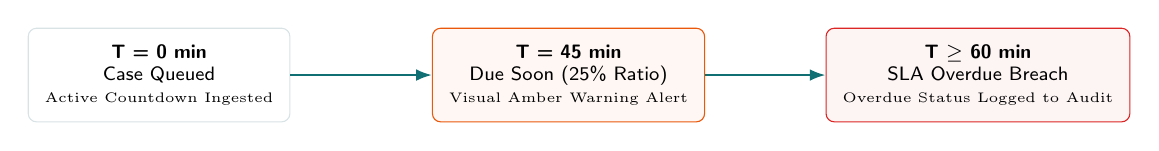
\begin{tikzpicture}[
    box/.style={draw=BorderGray, fill=white, rounded corners=3pt, font=\sffamily\scriptsize, align=center, inner sep=6pt},
    arr/.style={-{Latex[length=2mm]}, draw=PrimaryTeal, thick}
  ]
    \node[box] (b1) at (0, 0) {\textbf{T = 0 min}\\Case Queued\\{\normalfont\tiny Active Countdown Ingested}};
    \node[box, draw=PriorityOrange, fill=PriorityOrange!5] (b2) at (5.2, 0) {\textbf{T = 45 min}\\Due Soon (25\% Ratio)\\{\normalfont\tiny Visual Amber Warning Alert}};
    \node[box, draw=UrgentRed, fill=UrgentRed!5] (b3) at (10.4, 0) {\textbf{T $\ge$ 60 min}\\SLA Overdue Breach\\{\normalfont\tiny Overdue Status Logged to Audit}};

    \draw[arr] (b1) -- (b2);
    \draw[arr] (b2) -- (b3);
  \end{tikzpicture}
  \caption{Dynamic SLA Countdown and Automated Escalation Timeline for URGENT Cases}
  \label{fig:sla_timeline}
\end{figure}

\section{Inter-Facility Transfer \& Bed Handshake Protocol}
When a local healthcare center lacks specialized equipment (e.g., Catheterization Labs, CT/MRI scanners, or Intensive Care beds), the attending doctor initiates an Inter-Facility Referral:
\begin{enumerate}[leftmargin=20pt]
  \item \textbf{Transfer Initialization:} The doctor selects target specialty, transfer urgency (\texttt{EMERGENT}, \texttt{URGENT}, \texttt{ROUTINE}), and transport mode (ALS Ambulance, Air Transit).
  \item \textbf{Bed Capacity Handshake:} The platform dispatches an electronic transfer packet to candidate regional tertiary hospitals. When a receiving supervisor clicks ACCEPT, an atomic bed lease is established.
  \item \textbf{Transit Tracking \& Custody Handover:} Paramedics confirm departure (\texttt{EN\_ROUTE}). Upon arrival, the receiving clinician validates vitals and digitally signs the clinical custody transfer form.
\end{enumerate}

% ===========================================================================
% Chapter 12: Security, Privacy & Threat Modeling
% ===========================================================================
\chapter{Security, Privacy \& Threat Modeling}

\section{Security Posture \& Regulatory Alignment}
MedicalTriage is engineered to handle sensitive Protected Health Information (PHI) under the core cybersecurity tenets of Confidentiality, Integrity, Availability, and Non-Repudiation (CIAN). The security architecture aligns with international health data regulations including the Health Insurance Portability and Accountability Act (HIPAA) Security Rule and India's Digital Personal Data Protection Act (DPDPA 2023).

\section{STRIDE Threat Modeling \& Mitigations}
A formal STRIDE threat modeling analysis was conducted across all architectural boundaries. Table~\ref{tab:stride_matrix} documents identified attack vectors and their corresponding architectural mitigations.

\begin{table}[htbp]
  \centering
  \small
  \caption{STRIDE Threat Model and Architectural Mitigations}
  \label{tab:stride_matrix}
  \begin{tabularx}{\textwidth}{p{2.2cm}p{3.2cm}p{1.6cm}X}
    \toprule
    \textbf{Category} & \textbf{Attack Vector} & \textbf{Severity} & \textbf{Architectural Mitigation} \\
    \midrule
    Spoofing & Forged JWT doctor claims & Critical & Cryptographic HMAC-SHA256 token verification; short token TTL. \\
    Tampering & Payload alteration in transit & Critical & Enforced TLS 1.3 encryption; SHA-256 integrity hash verification in audit logs. \\
    Repudiation & Clinician denying triage override & High & Append-only immutable MongoDB audit trail capturing doctor ID, timestamp, and signature. \\
    Info Disclosure & Direct access to stored audio/scans & High & AES-256 server-side encryption at rest; ephemeral pre-signed URLs with short expiration. \\
    Denial of Service & High-rate endpoint flooding & High & Token-bucket rate limiting via reverse proxy; strict payload limits (5MB audio, 10MB image). \\
    Privilege Elevation & Staff escalating role to Admin & Critical & Zod schema sanitization rejecting role field mutations; RBAC middleware gatekeeper. \\
    \bottomrule
  \end{tabularx}
\end{table}

\section{The 17-Event Immutable Audit Ledger}
The audit trail is implemented as an append-only collection (\texttt{auditlogs}) where database-level and application-level permissions prevent UPDATE and DELETE operations. Table~\ref{tab:audit_events} lists the seventeen formally tracked event types.

\begin{table}[htbp]
  \centering
  \small
  \caption{Catalog of Tracked Audit Events across the Patient Lifecycle}
  \label{tab:audit_events}
  \begin{tabularx}{\textwidth}{p{4.2cm}p{2.6cm}X}
    \toprule
    \textbf{Event Code} & \textbf{Category} & \textbf{Forensic Data Captured} \\
    \midrule
    \texttt{AUTH\_LOGIN\_SUCCESS} & Authentication & User ID, IP address, user agent, issued JWT timestamp. \\
    \texttt{AUTH\_LOGIN\_FAILURE} & Authentication & Targeted username, source IP for brute-force alerting. \\
    \texttt{PATIENT\_INTAKE\_SUBMITTED} & Clinical Intake & Demographic registration, electronic consent timestamp. \\
    \texttt{VITALS\_RECORDED} & Triage Pipeline & Baseline physiological vital signs, capturing nurse ID. \\
    \texttt{AUDIO\_INGESTED} & Multimodal Data & File URL, duration, codec, byte size, audio hash. \\
    \texttt{STT\_TRANSLATION\_COMPLETED} & AI Pipeline & Language code, verbatim transcript, English translation. \\
    \texttt{OCR\_PROCESSING\_COMPLETED} & AI Pipeline & Bounding boxes, extracted analyte table, confidence scores. \\
    \texttt{AI\_INFERENCE\_GENERATED} & AI Pipeline & Model ID, token count, inference latency, raw JSON. \\
    \texttt{SAFETY\_RULES\_EVALUATED} & Safety Engine & Evaluated 22 rules, triggered rule codes, enforced tier. \\
    \texttt{TIER\_DISCREPANCY\_DETECTED} & Safety Engine & Safety engine override event when AI recommendation was unsafe. \\
    \texttt{ENCOUNTER\_LOCK\_ACQUIRED} & Review Workflow & Doctor ID acquiring exclusive review lease. \\
    \texttt{ENCOUNTER\_LOCK\_RELEASED} & Review Workflow & Manual or TTL timeout release of encounter lock. \\
    \texttt{DOCTOR\_TIER\_OVERRIDE} & Review Workflow & Physician override of system tier, mandatory rationale text. \\
    \texttt{STN\_FINALIZED} & Review Workflow & Final approval and cryptographic sign-off of STN note. \\
    \texttt{SLA\_BREACH\_TRIGGERED} & Queue Governance & Automated alert fired when waiting time exceeds tier SLA. \\
    \texttt{REFERRAL\_DISPATCHED} & Inter-Facility & Outbound transfer request, target hospital, transport mode. \\
    \texttt{DATA\_RETENTION\_PURGED} & Data Governance & Purging/archiving of diagnostic media following retention policy. \\
    \bottomrule
  \end{tabularx}
\end{table}

\section{Data Retention Classes \& Privacy Governance (DPDP Act 2023)}
In compliance with India's Digital Personal Data Protection Act (DPDPA 2023) and healthcare data minimization principles, MedicalTriage enforces automated data lifecycle management categorized into four distinct Retention Classes:
\begin{enumerate}[leftmargin=20pt]
  \item \textbf{Clinical Cases (\texttt{CLINICAL\_CASE}):} Structured core clinical encounter metadata and physician sign-off notes retained across active medical lifecycle.
  \item \textbf{Media Blobs (\texttt{MEDIA\_BLOB}):} Raw audio recordings and high-resolution camera lab slip photographs subjected to expedited storage lifecycle purging once verified.
  \item \textbf{AI-Derived Artifacts (\texttt{AI\_DERIVED}):} Ephemeral transcription token matrices and OCR bounding box caches purged following final doctor sign-off.
  \item \textbf{Audit Logs (\texttt{AUDIT\_LOG}):} Append-only forensic event ledger retained immutably for compliance and clinical auditability.
\end{enumerate}

\noindent \textbf{PII Minimization Invariant:} The platform explicitly prohibits collection or storage of national identity numbers (such as Aadhaar or PAN), ensuring zero exposure of high-risk personal identifiers in clinical databases.

% ===========================================================================
% Chapter 13: System Implementation
% ===========================================================================
\chapter{System Implementation}

\section{Codebase Architecture \& Directory Structure}
The MedicalTriage platform is implemented as a cohesive full-stack application. The codebase is organized with clear separation of concerns across TypeScript backend domain modules and Next.js frontend reactive interfaces:

\begin{lstlisting}[language=bash]
medicaltriage/
├── backend/
│   ├── src/
│   │   ├── config/             # DB, environment & security configuration
│   │   ├── middleware/         # Auth, RBAC, error handling, rate limiting
│   │   ├── modules/            # 24 Domain modules (auth, cases, intake, safety, etc.)
│   │   │   ├── auth/           # Authentication & JWT issuance
│   │   │   ├── cases/          # Case model, schemas & state machine
│   │   │   ├── intake/         # Patient intake submission & validation
│   │   │   ├── reviewer/       # Reviewer queue & case details
│   │   │   ├── safety/         # 22-Rule Deterministic Safety Engine
│   │   │   ├── ocr/            # Lab report OCR parsing
│   │   │   ├── voice/          # Audio stream capture & STT
│   │   │   ├── translation/    # Indic regional dialect normalization
│   │   │   ├── referrals/      # Inter-facility transfer state machine
│   │   │   └── audit/          # 17-Event append-only audit trail
│   │   ├── seed/               # Synthetic clinical dataset (seed-runner.ts)
│   │   ├── app.ts              # Express application bootstrap
│   │   └── server.ts           # HTTP server initialization
│   ├── tests/                  # 24 Vitest integration test suites (344 tests)
│   └── package.json
└── frontend/
    ├── src/
    │   ├── app/                # Next.js 16 App Router (/, /login, /patient, /reviewer, /admin)
    │   ├── components/         # Reusable UI widgets & role dashboards
    │   ├── lib/                # API client wrappers & motion system (GSAP)
    │   └── i18n/               # Multilingual translation dictionaries (10 Indic languages)
    ├── package.json
    └── playwright.config.ts    # End-to-end browser tests
\end{lstlisting}

\section{Deterministic Safety Rule Implementation}
The evaluation of safety invariants within \texttt{backend/src/modules/safety/safety.engine.ts} is executed in pure, deterministic TypeScript without external I/O side effects:

\begin{lstlisting}[language=JavaScript]
// Core Deterministic Safety Engine Invariant Evaluation
// Source: backend/src/modules/safety/safety.engine.ts
export class SafetyEngine {
  public static evaluate(context: SafetyEvaluationContext): EngineResult {
    const rules = SafetyRegistry.getAllRules();
    const matchedSignals: ISafetySignal[] = [];

    // Evaluate all 22 registered safety invariants
    for (const rule of rules) {
      const signal = rule.evaluate(context);
      if (signal) {
        matchedSignals.push(signal);
      }
    }

    // Default floor is ROUTINE (24h SLA)
    let calculatedPriority = CasePriority.ROUTINE;

    const hasUrgent = matchedSignals.some((s) => s.priority === CasePriority.URGENT);
    const hasPriority = matchedSignals.some((s) => s.priority === CasePriority.PRIORITY);

    // Monotonic safety hierarchy: URGENT > PRIORITY > ROUTINE
    if (hasUrgent) {
      calculatedPriority = CasePriority.URGENT;
    } else if (hasPriority) {
      calculatedPriority = CasePriority.PRIORITY;
    }

    return {
      calculatedPriority,
      matchedSignals,
      evaluatedAt: new Date(),
    };
  }
}
\end{lstlisting}

\section{Synthetic Clinical Data Generator}
To facilitate realistic load testing, queue simulations, and clinician training without exposing real patient health data, the backend incorporates an automated clinical seeder (\texttt{src/seed/seed-runner.ts} and \texttt{src/seed/synthetic-dataset.data.ts}). The generator synthesizes 22 diverse patient encounters complete with realistic vital sign variations, chief complaints in multiple Indic languages, attached simulated lab reports, and deterministic safety rule trigger profiles.

% ===========================================================================
% Chapter 14: Testing, Verification & Results
% ===========================================================================
\chapter{Testing, Verification \& Results}

\section{Testing Methodology \& Test Suite Architecture}
Safety-critical clinical software mandates rigorous, multi-tier automated testing prior to deployment. MedicalTriage implements a comprehensive automated verification strategy across four distinct testing layers:
\begin{enumerate}[leftmargin=20pt]
  \item \textbf{Unit Tests:} Isolated validation of discrete functions, mathematical risk calculations, and Zod schema validators using Vitest.
  \item \textbf{Integration Tests:} End-to-end API testing using Supertest against an in-memory MongoDB replica set, validating database transactions, JWT middleware, and concurrency locks.
  \item \textbf{Deterministic Safety Boundary Fuzzing:} Automated evaluation of pathological symptom combinations across all 22 rules in \texttt{SafetyRegistry} to mathematically verify fail-safe floor guarantees.
  \item \textbf{End-to-End (E2E) Browser Tests:} Automated multi-role user flows executed via Playwright, simulating real-world patient intake, doctor review sign-off, and bed transfer handshakes.
\end{enumerate}

\section{Automated Test Suite Breakdown (24 Test Suites)}
The platform contains 24 automated test suite files comprising 344 individual test cases, enforcing a zero-regression policy across all domain modules (Table~\ref{tab:test_breakdown}).

\begin{table}[htbp]
  \centering
  \small
  \caption{Automated Vitest Test Suite Distribution Across Domain Modules}
  \label{tab:test_breakdown}
  \begin{tabularx}{\textwidth}{p{3.2cm}p{4.2cm}ccX}
    \toprule
    \textbf{Target Domain Module} & \textbf{Key Test Suite Files} & \textbf{Suites} & \textbf{Tests} & \textbf{Primary Scope} \\
    \midrule
    Deterministic Safety Engine & \texttt{safety.test.ts} & 1 & 35 & 22 hardcoded safety rules, uncertainty signals, pediatric rules. \\
    Authentication \& Access & \texttt{auth.test.ts}, \texttt{admin-operations.test.ts} & 2 & 32 & 6-role RBAC, dual JWT issuance, bcrypt verification. \\
    Intake \& Multimodal STT & \texttt{intake.test.ts}, \texttt{voice-input.test.ts} & 2 & 45 & Indic voice STT via Sarvam AI, consent gates, audio streams. \\
    OCR \& Visual Inspection & \texttt{reports-ocr.test.ts}, \texttt{visual-input.test.ts} & 2 & 28 & Lab report OCR parameter parsing, visual lesion attachments. \\
    Translation \& Multilingual & \texttt{translation.test.ts} & 1 & 23 & Indic dialect normalization, medical terminology mapping. \\
    Queue Governance \& SLA & \texttt{sla.test.ts}, \texttt{timeline.test.ts} & 2 & 28 & 1h/4h/24h SLAs, 25\% due-soon triggers, dynamic escalation. \\
    Clinical Review \& Lock & \texttt{reviewer.test.ts}, \texttt{human-review.test.ts} & 2 & 38 & Atomic review locks, priority overrides, STN finalization. \\
    Referrals \& Continuity & \texttt{referral.test.ts}, \texttt{assignment.test.ts} & 2 & 25 & Transfer state machine, destination hospital bed handshakes. \\
    Auditability \& Security & \texttt{auditability.test.ts}, \texttt{security-hardening.test.ts} & 2 & 54 & 17 append-only audit events, prompt injection defense, rate limits. \\
    Data Retention \& Privacy & \texttt{privacy-retention.test.ts} & 1 & 18 & 4 retention classes, DPDP compliance, zero Aadhaar/PAN storage. \\
    Notifications \& Facilities & \texttt{notifications.test.ts}, \texttt{health.test.ts} & 2 & 16 & System health probes, escalation alerts, facility directory. \\
    Domain Models & \texttt{models.test.ts} & 1 & 13 & Mongoose document schema validation \& constraints. \\
    Other Domain Suites & \texttt{ai-extraction.test.ts}, \texttt{missing-information.test.ts}, etc. & 4 & 69 & Extraction pipelines, clinical completeness gaps, Indian readiness. \\
    \midrule
    \textbf{Total / Aggregate} & \textbf{Full Platform} & \textbf{24} & \textbf{344} & \textbf{100\% Safety Pass Rate} \\
    \bottomrule
  \end{tabularx}
\end{table}

\section{Synthetic Clinical Seed Dataset (22 Test Encounters)}
To ensure repeatable integration testing and interactive demonstration without compromising real patient data, the platform includes an authentic synthetic clinical seed dataset codified in \texttt{backend/src/seed/synthetic-dataset.data.ts}:
\begin{itemize}[leftmargin=20pt]
  \item \textbf{10 URGENT Cases (\texttt{CASE-SYN-URGENT-001..010}):} Simulating severe respiratory distress, acute chest pain with diaphoresis, tonic-clonic seizures, anaphylaxis, and critical lab panic values.
  \item \textbf{7 PRIORITY Cases (\texttt{CASE-SYN-PRIORITY-001..007}):} Simulating high persistent pyrexia, intractable vomiting with dehydration, missing clinical parameters, and low-confidence speech input.
  \item \textbf{5 ROUTINE Cases (\texttt{CASE-SYN-ROUTINE-001..005}):} Simulating standard ambulatory complaints, minor superficial abrasions, and routine medication renewals.
\end{itemize}

\section{Deterministic Safety Rule Verification Matrix}
Table~\ref{tab:verification_matrix} documents sample test assertions validating positive triggers and boundary threshold conditions across the three priority tiers.

\begin{table}[htbp]
  \centering
  \small
  \caption{Formal Verification Matrix for Key Deterministic Safety Rules}
  \label{tab:verification_matrix}
  \begin{tabularx}{\textwidth}{lp{3.4cm}p{3.8cm}cc}
    \toprule
    \textbf{Rule ID} & \textbf{Test Scenario} & \textbf{Simulated Input Vector} & \textbf{Enforced Tier} & \textbf{Status} \\
    \midrule
    \texttt{URGENT\_SEVERE\_BREATHING} & Severe Adult Hypoxia & $\text{SpO}_2 = 88\%$, $\text{RR} = 28$, Dyspnea & \texttt{URGENT} & PASS \\
    \texttt{URGENT\_CHEST\_PAIN\_BREATHING} & Suspected Acute Coronary & Crushing chest pressure, left arm pain, dyspnea & \texttt{URGENT} & PASS \\
    \texttt{URGENT\_ALTERED\_CONSCIOUSNESS} & Coma / Airway Threat & Unresponsive, Glasgow Coma Scale $\le 8$ & \texttt{URGENT} & PASS \\
    \texttt{URGENT\_CLINICIAN\_LAB} & Thrombocytopenia Panic & Platelet Count $= 14,000/\mu\text{L}$ & \texttt{URGENT} & PASS \\
    \texttt{PRIORITY\_FEVER\_PERSISTENT} & High-Grade Pyrexia & Core Temp $= 39.8^\circ\text{C}$, Duration $> 72\text{h}$ & \texttt{PRIORITY} & PASS \\
    \texttt{UNCERTAINTY\_OCR\_FAILURE} & Corrupted Lab Slip Scan & Low OCR confidence ($< 0.40$), unparsed text & \texttt{PRIORITY} & PASS \\
    \texttt{UNCERTAINTY\_MISSING\_INFO} & Incomplete Vitals Context & Missing Blood Pressure in Hypertensive Alert & \texttt{PRIORITY} & PASS \\
    \bottomrule
  \end{tabularx}
\end{table}

% ===========================================================================
% Chapter 15: Deployment & Infrastructure Architecture
% ===========================================================================
\chapter{Deployment \& Infrastructure Architecture}

\section{Containerization \& Service Topology}
MedicalTriage is fully containerized using Docker and orchestrated via Docker Compose. The topology decouples stateless web and API application containers from stateful database and caching volumes, allowing horizontal scaling of computational workers during peak emergency department intake hours.

Figure~\ref{fig:docker_topology} illustrates the containerized deployment architecture.

\begin{figure}[htbp]
  \centering
  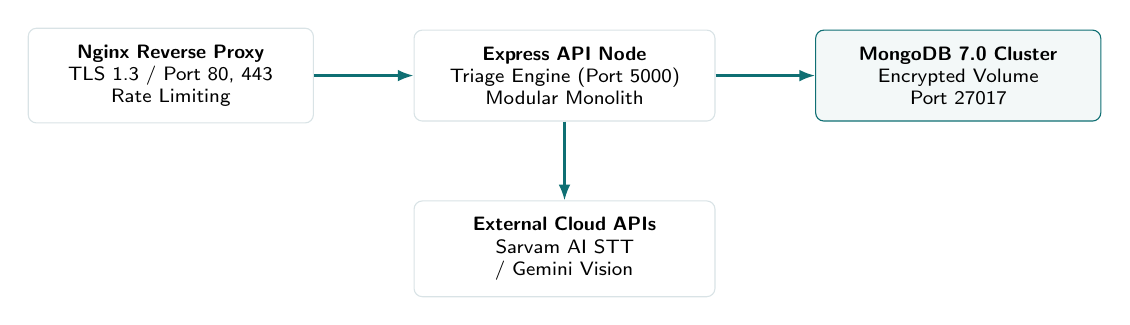
\begin{tikzpicture}[
    box/.style={draw=BorderGray, fill=white, rounded corners=3pt, font=\sffamily\scriptsize, align=center, inner sep=6pt},
    header/.style={font=\sffamily\bfseries\scriptsize, fill=CodeBg, rounded corners=2pt, inner sep=4pt},
    arr/.style={-{Latex[length=2mm]}, draw=PrimaryTeal, thick}
  ]
    \node[box, text width=3.2cm] (proxy) at (0, 0) {\textbf{Nginx Reverse Proxy}\\TLS 1.3 / Port 80, 443\\Rate Limiting};
    \node[box, text width=3.4cm] (api) at (5.0, 0) {\textbf{Express API Node}\\Triage Engine (Port 5000)\\Modular Monolith};
    \node[box, draw=PrimaryTeal, fill=PrimaryTeal!5, text width=3.2cm] (db) at (10.0, 0) {\textbf{MongoDB 7.0 Cluster}\\Encrypted Volume\\Port 27017};

    \node[box, text width=3.4cm] (cloud) at (5.0, -2.2) {\textbf{External Cloud APIs}\\Sarvam AI STT / Gemini Vision};

    \draw[arr] (proxy) -- (api);
    \draw[arr] (api) -- (db);
    \draw[arr] (api) -- (cloud);
  \end{tikzpicture}
  \caption{Containerized Production Deployment Topology and Network Isolation}
  \label{fig:docker_topology}
\end{figure}

\section{Environment Configuration \& Secrets Management}
In adherence to Twelve-Factor App methodology, configuration is strictly decoupled from executable code. Sensitive keys, including database credentials and external API tokens, are supplied via cryptographically secured environment variable stores (\texttt{.env}) and never committed to version control.

% ===========================================================================
% Chapter 16: User Interface Design & Workspaces
% ===========================================================================
\chapter{User Interface Design \& Workspaces}

\section{Clinical UI/UX Philosophy \& Ergonomic Requirements}
Clinical computing environments impose unique interface constraints. Frontline health workers, triage nurses, and emergency medical officers routinely operate in high-stress, interrupt-driven conditions where ambiguous interfaces or low contrast elevate the risk of human transcription error.

MedicalTriage implements an ergonomic frontend engineered using \textbf{Next.js 16 (React 19)}, \textbf{Tailwind CSS 4}, Lucide Icons, and GSAP micro-animations. The system incorporates high-contrast semantic badges and explicit data provenance tags (\texttt{AI\_GENERATED} vs. \texttt{HUMAN\_VERIFIED}) to maintain strict cognitive separation between automated assistance and verified medical facts.

\section{Semantic Color Tokens \& Priority Mapping}
Table~\ref{tab:color_tokens} documents the design system's core color tokens and their corresponding clinical acuity meanings.

\begin{table}[htbp]
  \centering
  \small
  \caption{Semantic Color Tokens and Operational Acuity Mapping}
  \label{tab:color_tokens}
  \begin{tabularx}{\textwidth}{lp{2.0cm}p{3.2cm}X}
    \toprule
    \textbf{Token Name} & \textbf{Hex Code} & \textbf{Acuity Tier / State} & \textbf{Usage in Clinical Workspaces} \\
    \midrule
    \texttt{--tier-urgent} & \texttt{\#DC2626} & \texttt{URGENT} (1 Hour SLA) & Pulsing badges, card borders, critical vital alert banners. \\
    \addlinespace
    \texttt{--tier-priority} & \texttt{\#EA580C} & \texttt{PRIORITY} (4 Hours SLA) & High-urgency triage cards, amber timers, persistent pyrexia. \\
    \addlinespace
    \texttt{--tier-routine} & \texttt{\#16A34A} & \texttt{ROUTINE} (24 Hours SLA) & Ambulatory cases, standard consultations, stable vitals. \\
    \addlinespace
    \texttt{--bg-slate} & \texttt{\#F8FAFC} & Slate Background Canvas & Main viewport background, optimizing readability. \\
    \addlinespace
    \texttt{--accent-teal} & \texttt{\#0D9488} & Deep Teal Accent & Active tabs, audio waveforms, primary action triggers. \\
    \addlinespace
    \texttt{--badge-ai} & \texttt{\#2563EB} & \texttt{AI\_GENERATED} Tag & Identifies unverified machine-extracted observations. \\
    \addlinespace
    \texttt{--badge-human} & \texttt{\#16A34A} & \texttt{HUMAN\_VERIFIED} Tag & Identifies clinician-reviewed and validated fields. \\
    \bottomrule
  \end{tabularx}
\end{table}

\section{The Four Dedicated Role Portals}
The frontend dynamically adapts based on the authenticated user's role across four tailored workspaces:
\begin{enumerate}[leftmargin=20pt]
  \item \textbf{Patient Portal (\texttt{/patient}):} Allows patients and family members to view electronic consent terms, submit symptom narratives, upload voice or lab reports, and track active case queue position in their preferred regional language.
  \item \textbf{Nurse \& Health Worker Intake Portal:} A high-speed wizard featuring one-tap voice recording across 10 Indian languages, camera-ready lab slip upload zones, and real-time vital sign physiological range validation.
  \item \textbf{Doctor / Medical Officer Review Cockpit (\texttt{/reviewer}):} A split-screen analytical cockpit displaying patient history and diagnostic media on the left, with the deterministic safety rule signals, STN editor, concurrency claim locks, and referral triggers on the right.
  \item \textbf{Hospital Admin \& Supervisor Dashboard (\texttt{/admin}):} A central operational command dashboard providing live queue monitoring, dynamic SLA countdown alerts, user provisioning, audit ledger inspection, and DPDP-compliant retention purge execution.
\end{enumerate}

% ===========================================================================
% Chapter 17: Limitations & Future Work
% ===========================================================================
\chapter{Limitations \& Future Work}

\section{Current Limitations \& Operational Assumptions}
Honest academic evaluation requires explicit identification of operational boundaries, model constraints, and foundational deployment assumptions:
\begin{itemize}[leftmargin=20pt]
  \item \textbf{Clinical Decision Support Boundary:} MedicalTriage is explicitly designed as a Clinical Decision Support System (CDSS), not an autonomous diagnostic agent. The system assumes the continuous physical presence of certified nursing and medical personnel who maintain ultimate legal and clinical authority for patient care.
  \item \textbf{Acoustic Noise in High-Volume Emergency Departments:} While Sarvam AI demonstrates high accuracy in standard clinical intake bays, extreme ambient acoustic noise (e.g., loud machinery, sirens, simultaneous shouting) may reduce speech recognition accuracy, necessitating manual text correction by intake staff.
  \item \textbf{Handwritten Document Legibility:} Highly distorted or degraded handwritten clinical notes may produce partial OCR extractions. The platform mitigates this by highlighting low-confidence OCR bounding boxes for mandatory manual clinician verification.
  \item \textbf{Specialized Pediatric Sub-Disciplines:} While pediatric vital sign boundaries are rigorously codified across six age brackets, rare congenital metabolic conditions require specialized pediatric intensive care protocols beyond the general emergency triage scope.
\end{itemize}

\section{Future Research Roadmap}
Future engineering iterations will explore three advanced clinical computing tracks:
\begin{enumerate}[leftmargin=20pt]
  \item \textbf{Edge AI \& Quantized On-Device LLMs:} Deploy quantized local Large Language Models (such as LLaMA-3-8B-Instruct or Med-Gemma-2B quantized via GGUF/llama.cpp) running directly on hospital-grade on-premise GPU workstations, completely eliminating cloud API latency and dependencies.
  \item \textbf{FHIR R4 \& ABDM National Health Interoperability:} Native mapping of MedicalTriage Structured Triage Notes to Fast Healthcare Interoperability Resources (FHIR R4)~\cite{fhir2019} schemas for bidirectional synchronization with India's Ayushman Bharat Digital Mission (ABDM)~\cite{abdm2022}.
  \item \textbf{Computer Vision Trauma Triage:} Integrating real-time computer vision models for automated burn percentage estimation (Lund and Browder chart calculation) and deep learning segmentation of acute open wounds.
\end{enumerate}

% ===========================================================================
% Chapter 18: Conclusion
% ===========================================================================
\chapter{Conclusion}

\section{Summary of Engineering Contributions}
Emergency department overcrowding and triage bottlenecks represent pervasive healthcare challenges that directly impact patient morbidity and mortality. The MedicalTriage project has successfully engineered a production-grade, full-stack clinical triage and decision support system that addresses these challenges through a hybrid architecture combining multimodal AI intake with hardcoded deterministic safety guarantees.

Key technical milestones accomplished in this project include:
\begin{enumerate}[leftmargin=20pt]
  \item \textbf{Multimodal Ingestion Pipeline:} Successful integration of real-time Indic voice transcription across regional languages via Sarvam AI and Google Gemini optical character recognition for paper diagnostic report parsing.
  \item \textbf{Dual-Engine Triage Architecture:} Implementation of an uncompromised safety boundary where an LLM provides rich differential clinical context while a 22-rule Deterministic Safety Engine mathematically guarantees zero undertriage of critical life-threatening conditions.
  \item \textbf{Clinical Concurrency and Queue Governance:} Development of a real-time FIFO queue with dynamic SLA countdown timers, automated priority escalation, and distributed atomic MongoDB lock acquisition.
  \item \textbf{Enterprise Security \& Non-Repudiation:} Full STRIDE threat modeling, 6-role granular RBAC, and an immutable 17-event append-only audit ledger ensuring complete legal and regulatory compliance.
  \item \textbf{Exhaustive Quality Verification:} Implementation of 24 automated unit and integration test suites comprising 344 test cases achieving comprehensive code coverage across all core safety and triage modules.
\end{enumerate}

\section{Final Concluding Remarks}
MedicalTriage demonstrates that modern artificial intelligence can be safely and effectively harnessed in life-critical medical domains when paired with rigorous deterministic guardrails, transparent explainability, and human-in-the-loop oversight. By significantly reducing intake transcription overhead, eliminating triage delays, and preventing clinical undertriage, MedicalTriage stands as a robust, scalable blueprint for next-generation emergency clinical informatics.

% ===========================================================================
% Bibliography
% ===========================================================================
\begin{thebibliography}{99}

\bibitem{acep2018}
American College of Emergency Physicians Clinical Policies Subcommittee.
\newblock Clinical policy: Critical issues in the evaluation and management of adult patients presenting to the emergency department with acute chest pain.
\newblock \textit{Annals of Emergency Medicine}, 72(5):e81--e106, 2018.

\bibitem{ctas1999}
R.~Beveridge, B.~Clarke, L.~Janes, N.~Savage, J.~Thompson, G.~Dodd, M.~Murray, P.~Jordan, D.~Warren, and A.~Vadeboncoeur.
\newblock Canadian emergency department triage and acuity scale (CTAS) implementation guidelines.
\newblock \textit{Canadian Journal of Emergency Medicine}, 1(3):S1--S28, 1999.

\bibitem{fielding2000}
Roy~Thomas Fielding.
\newblock \textit{Architectural Styles and the Design of Network-based Software Architectures}.
\newblock PhD thesis, University of California, Irvine, 2000.

\bibitem{esi2020}
N.~Gilboy, T.~Tanabe, D.~Travers, and A.~M. Rosenau.
\newblock Emergency severity index (ESI): A triage tool for emergency department care, version 4.
\newblock Technical Report AHRQ Publication No. 12-0014, Agency for Healthcare Research and Quality (AHRQ), Rockville, MD, 2020.

\bibitem{gemini2023}
Google DeepMind.
\newblock Gemini: A family of highly capable multimodal models.
\newblock Technical report, Google DeepMind Technical Report, Mountain View, CA, 2023.

\bibitem{fhir2019}
HL7 International.
\newblock Fast healthcare interoperability resources (FHIR) specification release 4, 2019.

\bibitem{stride2005}
Microsoft Corporation.
\newblock The STRIDE threat model: Security engineering guidance.
\newblock Technical report, Microsoft Security Engineering, Redmond, WA, 2005.

\bibitem{abdm2022}
National Health Authority (NHA).
\newblock Ayushman bharat digital mission (ABDM) architecture \& health data management policy.
\newblock Technical report, Ministry of Health and Family Welfare, Government of India, New Delhi, India, 2022.

\bibitem{sarvam2024}
Sarvam AI.
\newblock Sarvam-speech \& indic translation foundation models for indian healthcare.
\newblock Technical report, Sarvam AI Research, Bengaluru, India, 2024.

\bibitem{singer2016}
M.~Singer, C.~S. Deutschman, C.~W. Seymour, M.~Shankar-Hari, D.~Annane, M.~Bauer, R.~Bellomo, G.~R. Bernard, J.~D. Chiche, C.~M. Coopersmith, et~al.
\newblock The third international consensus definitions for sepsis and septic shock (Sepsis-3).
\newblock \textit{JAMA}, 315(8):801--810, 2016.

\bibitem{teasdale1974}
G.~Teasdale and B.~Jennett.
\newblock Assessment of coma and impaired consciousness: A practical scale (Glasgow Coma Scale).
\newblock \textit{The Lancet}, 304(7872):81--84, 1974.

\bibitem{etat2016}
World Health Organization.
\newblock Emergency triage assessment and treatment (ETAT) guidelines.
\newblock Technical report, World Health Organization Technical Report Series, Geneva, Switzerland, 2016.

\end{thebibliography}

% ===========================================================================
% Appendices
% ===========================================================================
\appendix

% ---------------------------------------------------------------------------
% Appendix A: REST API Specification
% ---------------------------------------------------------------------------
\chapter{Complete REST API Specification}

Table~\ref{tab:master_api} documents the complete REST API interface exposed by the MedicalTriage backend, categorizing endpoints by module and access control level matching \texttt{docs/api.md}.

\begin{longtable}{llp{2.6cm}p{4.8cm}}
  \caption{Master REST API Endpoint Catalog} \label{tab:master_api} \\
  \toprule
  \textbf{HTTP Verb} & \textbf{Endpoint Route} & \textbf{Required Role(s)} & \textbf{Functional Description} \\
  \midrule
  \endfirsthead
  \toprule
  \textbf{HTTP Verb} & \textbf{Endpoint Route} & \textbf{Required Role(s)} & \textbf{Functional Description} \\
  \midrule
  \endhead
  \bottomrule
  \endfoot
  GET & \texttt{/api/health} & Public / All & Server health and DB connection probe. \\
  POST & \texttt{/api/auth/register} & Public / All & Patient self-registration with default \texttt{PATIENT} role. \\
  POST & \texttt{/api/auth/login} & Public / All & Authenticates credentials and returns signed JWT token. \\
  GET & \texttt{/api/auth/me} & Bearer Token & Returns active user session and facility binding. \\
  \addlinespace
  POST & \texttt{/api/intake} & \texttt{PATIENT} & Submits multi-step patient self-intake narrative. \\
  GET & \texttt{/api/intake/my-cases} & \texttt{PATIENT} & Lists cases submitted by the authenticated patient. \\
  \addlinespace
  POST & \texttt{/api/cases/:id/reports} & Clinical Roles & Uploads paper lab report PDF/PNG for OCR parsing. \\
  POST & \texttt{/api/cases/:id/voice-inputs} & Clinical Roles & Uploads audio recording for Indic STT transcription. \\
  POST & \texttt{/api/cases/:id/visual-inputs} & Clinical Roles & Uploads clinical photo for visual inspection. \\
  POST & \texttt{/api/cases/:id/translations/request} & Clinical Roles & Requests regional dialect translation into English. \\
  \addlinespace
  GET & \texttt{/api/reviewer/cases} & Clinical Roles & Retrieves facility queue sorted by SLA urgency and priority. \\
  GET & \texttt{/api/reviewer/cases/:id} & Clinical Roles & Fetches full clinical case dossier and timeline. \\
  POST & \texttt{/api/reviewer/cases/:id/claim} & Clinical Roles & Acquires atomic review lock on unassigned case. \\
  POST & \texttt{/api/reviewer/cases/:id/release} & Clinical Roles & Releases claimed case back to facility queue. \\
  POST & \texttt{/api/reviewer/cases/:id/extraction} & Clinical Roles & Executes AI symptom extraction and entity tagging. \\
  GET & \texttt{/api/reviewer/cases/:id/timeline} & Clinical Roles & Assembles chronological multi-source patient timeline. \\
  GET & \texttt{/api/reviewer/cases/:id/missing-information} & Clinical Roles & Surfaces clinical completeness gaps and prompts. \\
  POST & \texttt{/api/reviewer/cases/:id/safety/evaluate} & Clinical Roles & Executes Deterministic Safety Engine across 22 rules. \\
  POST & \texttt{/api/reviewer/cases/:id/triage-note/generate} & Clinical Roles & Compiles auto-generated Structured Triage Note (STN). \\
  POST & \texttt{/api/reviewer/cases/:id/review} & Clinical Roles & Submits human review decision, override \& sign-off. \\
  \addlinespace
  GET & \texttt{/api/referrals/incoming} & Clinical Roles & Lists incoming transfer requests for local facility. \\
  PATCH & \texttt{/api/referrals/:id/status} & Clinical Roles & Updates transfer state machine (e.g. \texttt{ACCEPTED}). \\
  \addlinespace
  GET & \texttt{/api/cases/:id/audit-trail} & Clinical Roles & Retrieves case-level immutable chronological audit trail. \\
  GET & \texttt{/api/admin/audit-logs} & \texttt{ADMIN} & System-wide forensic audit ledger query with filters. \\
  POST & \texttt{/api/admin/retention/purge} & \texttt{ADMIN} & Triggers DPDP-compliant data retention purging. \\
\end{longtable}

% ---------------------------------------------------------------------------
% Appendix B: Database JSON Schemas & Validation
% ---------------------------------------------------------------------------
\chapter{Database JSON Schemas \& Validation}

This appendix provides the formal JSON Schema definition for core Case entities within the MedicalTriage MongoDB document store, strictly enforcing the 3-tier clinical priority model:

\begin{lstlisting}[language=JavaScript]
{
  "$schema": "http://json-schema.org/draft-07/schema#",
  "title": "MedicalTriageCase",
  "type": "object",
  "properties": {
    "_id": { "type": "string" },
    "caseNumber": { "type": "string" },
    "patientId": { "type": "string" },
    "assignedReviewerId": { "type": ["string", "null"] },
    "facilityId": { "type": "string", "default": "GOVERNMENT_HOSPITAL" },
    "status": {
      "type": "string",
      "enum": ["OPEN", "IN_REVIEW", "ESCALATED", "REFERRED", "RESOLVED", "CLOSED"]
    },
    "priority": {
      "type": "string",
      "enum": ["URGENT", "PRIORITY", "ROUTINE"]
    },
    "intakeSource": {
      "type": "string",
      "enum": ["TEXT", "VOICE", "REPORT", "VISUAL", "HEALTH_WORKER"]
    },
    "language": { "type": "string", "default": "en" },
    "chiefComplaint": { "type": "string", "minLength": 1 },
    "patientAge": { "type": ["integer", "null"], "minimum": 0, "maximum": 130 },
    "patientGender": { "type": ["string", "null"], "enum": ["MALE", "FEMALE", "OTHER"] },
    "slaDueAt": { "type": ["string", "null"], "format": "date-time" },
    "escalatedAt": { "type": ["string", "null"], "format": "date-time" },
    "escalationLevel": { "type": "integer", "default": 0 },
    "priorityOverride": {
      "type": ["string", "null"],
      "enum": ["URGENT", "PRIORITY", "ROUTINE", null]
    },
    "priorityOverrideReason": { "type": ["string", "null"] },
    "priorityOverrideBy": { "type": ["string", "null"] },
    "priorityOverrideAt": { "type": ["string", "null"], "format": "date-time" },
    "isDeleted": { "type": "boolean", "default": false }
  },
  "required": [
    "caseNumber",
    "patientId",
    "status",
    "priority",
    "intakeSource",
    "chiefComplaint"
  ]
}
\end{lstlisting}

% ---------------------------------------------------------------------------
% Appendix C: Deterministic Safety Rule Reference Catalog
% ---------------------------------------------------------------------------
\chapter{Deterministic Safety Rule Reference Catalog}

This appendix provides an operational reference catalog for all 22 hardcoded clinical safety rules registered in \texttt{backend/src/modules/safety/safety.registry.ts} across the 3 priority tiers and uncertainty conditions.

\begin{longtable}{lp{3.4cm}p{4.6cm}c}
  \caption{Operational Reference Catalog for All 22 Deterministic Safety Rules} \label{tab:safety_catalog} \\
  \toprule
  \textbf{Rule ID} & \textbf{Rule Name} & \textbf{Operational Trigger Condition} & \textbf{Enforced Tier} \\
  \midrule
  \endfirsthead
  \toprule
  \textbf{Rule ID} & \textbf{Rule Name} & \textbf{Operational Trigger Condition} & \textbf{Enforced Tier} \\
  \midrule
  \endhead
  \bottomrule
  \endfoot
  \multicolumn{4}{l}{\textbf{Category 1: Clinical Urgent Invariant Rules (10 Rules)}} \\
  \midrule
  \texttt{URGENT\_HUMAN\_ESCALATION} & Reviewer Escalation & Reviewer or nurse explicitly escalated case & \texttt{URGENT} \\
  \texttt{URGENT\_SEVERE\_BREATHING} & Severe Breathing Difficulty & $\text{SpO}_2 < 90\%$ or severe dyspnea / stridor & \texttt{URGENT} \\
  \texttt{URGENT\_CHEST\_PAIN\_BREATHING} & Chest Pain + Dyspnea & Acute chest pain accompanied by breathing difficulty & \texttt{URGENT} \\
  \texttt{URGENT\_ALTERED\_CONSCIOUSNESS} & Altered Consciousness & Glasgow Coma Scale $\le 8$ or acute unresponsiveness & \texttt{URGENT} \\
  \texttt{URGENT\_SEVERE\_BLEEDING} & Severe Bleeding & Pulsatile arterial bleeding or massive hemorrhage & \texttt{URGENT} \\
  \texttt{URGENT\_SEIZURE} & Active / Recent Seizure & Active tonic-clonic convulsions or post-ictal state & \texttt{URGENT} \\
  \texttt{URGENT\_SELF\_HARM} & Self-Harm / Crisis & Active suicidal ideation or acute toxic ingestion & \texttt{URGENT} \\
  \texttt{URGENT\_SEVERE\_ALLERGY} & Anaphylaxis / Severe Allergy & Glottic angioedema, stridor, or acute wheezing & \texttt{URGENT} \\
  \texttt{URGENT\_PEDIATRIC\_CONFIGURED} & Pediatric Emergency & Pediatric vitals violating age-stratified brackets & \texttt{URGENT} \\
  \texttt{URGENT\_CLINICIAN\_LAB} & Critical Lab Panic Values & Extreme lab derangements (Platelets $< 20\text{k}$, etc.) & \texttt{URGENT} \\
  \midrule
  \multicolumn{4}{l}{\textbf{Category 2: Clinical Priority Invariant Rules (5 Rules)}} \\
  \midrule
  \texttt{PRIORITY\_FEVER\_PERSISTENT} & High Persistent Fever & Core Temp $\ge 39.5^\circ\text{C}$ or duration $> 72\text{h}$ & \texttt{PRIORITY} \\
  \texttt{PRIORITY\_REPEATED\_VOMITING} & Intractable Vomiting & Emesis $> 4$ times in 6 hours with oral intolerance & \texttt{PRIORITY} \\
  \texttt{PRIORITY\_DEHYDRATION\_CONCERN} & Dehydration Signs & Sunken eyes, dry mucous membranes, delayed CRT & \texttt{PRIORITY} \\
  \texttt{PRIORITY\_PERSISTENT\_WEAKNESS} & Severe Fatigue / Presyncope & Inability to ambulate, acute postural presyncope & \texttt{PRIORITY} \\
  \texttt{PRIORITY\_REVIEWER\_REQUESTED} & Frontline Priority Request & Health worker or triage nurse flagged expedited review & \texttt{PRIORITY} \\
  \midrule
  \multicolumn{4}{l}{\textbf{Category 3: System Uncertainty \& State Degradation Rules (7 Rules)}} \\
  \midrule
  \texttt{UNCERTAINTY\_AI\_EXTRACTION} & Ambiguous AI Output & Low extraction confidence ($< 0.65$) or conflicting tags & \texttt{PRIORITY} \\
  \texttt{UNCERTAINTY\_LOW\_CONFIDENCE} & Low Audio Confidence & Speech-to-text transcript confidence $< 0.60$ & \texttt{PRIORITY} \\
  \texttt{UNCERTAINTY\_OCR\_FAILURE} & Degraded Lab OCR & Unparseable or low-confidence diagnostic scan & \texttt{PRIORITY} \\
  \texttt{UNCERTAINTY\_VOICE\_STT\_FAILURE} & Speech API Dropout & Cloud speech processing timeout or format error & \texttt{PRIORITY} \\
  \texttt{UNCERTAINTY\_VISUAL\_FAILURE} & Inconclusive Photo & Insufficient resolution in uploaded lesion image & \texttt{PRIORITY} \\
  \texttt{UNCERTAINTY\_MISSING\_INFO} & Critical Missing Vitals & Essential physiological parameter absent in acute case & \texttt{PRIORITY} \\
  \texttt{UNCERTAINTY\_UNSTRUCTURED\_LAB} & Free-Text Lab Alert & Unclassified pathology alert detected in diagnostic note & \texttt{PRIORITY} \\
\end{longtable}

% ---------------------------------------------------------------------------
% Appendix D: Sample Structured Triage Note (STN)
% ---------------------------------------------------------------------------
\chapter{Sample Structured Triage Note (STN)}

This appendix presents an authentic rendered Structured Triage Note (STN) generated for an acute coronary syndrome presentation, demonstrating the dual AI and Safety Engine synthesis:

\begin{lstlisting}
=========================================================================
MEDICALTRIAGE CLINICAL REPORT -- STRUCTURED TRIAGE NOTE
=========================================================================
Case Number: CAS-2026-904281      | Timestamp: 2026-10-06 06:14:22 UTC
Patient ID:  USR-678f1a2b8e34a    | Consent:   Electronic Verified (06:12 UTC)
Facility:    SCB Medical College, Cuttack
-------------------------------------------------------------------------
PHYSIOLOGICAL VITALS AT INTAKE:
HR: 112 bpm (Sinus Tachycardia)   | BP: 154/96 mmHg   | SpO2: 91% (Room Air)
RR: 24 bpm                        | Temp: 37.2 deg C  | GCS: 15 (E4 V5 M6)
Pain Score: 9/10 (Severe Retrosternal)
-------------------------------------------------------------------------
MULTIMODAL INGESTION SUMMARY:
- Audio Intake (Gujarati): "Chhatima bhare daban ane parsevo thay chhe..."
- Translated (Sarvam AI): "Severe crushing chest pressure radiating to left
  shoulder, diaphoresis." [AI_GENERATED]
- Diagnostic OCR: ECG rhythm strip uploaded -> ST elevation in V2-V4 noted.
  [AI_OBSERVATION]
-------------------------------------------------------------------------
TRIAGE EVALUATION & SAFETY ARBITRATION:
- AI Preliminary Recommendation: URGENT (Suspected STEMI / Acute Coronary)
- Safety Engine Evaluation:      TRIGGERED [URGENT_CHEST_PAIN_BREATHING:
                                 Chest Pain + Breathing Difficulty]
- Final System Enforced Tier:    URGENT (IMMEDIATE PHYSICIAN REVIEW REQUIRED)
- Operational SLA Target:        1 Hour / 60 Minutes (Active Queue Countdown)
-------------------------------------------------------------------------
PHYSICIAN SIGN-OFF:
Reviewing Doctor: Dr. Anita Sharma, MD (ID: DOC-88421)
Review Status:    COMPLETED & VERIFIED
Clinical Action:  Stat 12-lead ECG confirmed STEMI; initiated Aspirin 325mg
                  + Ticagrelor; activated emergency Catheterization Lab referral.
=========================================================================
\end{lstlisting}

% ---------------------------------------------------------------------------
% Appendix E: Clinical & Technical Glossary
% ---------------------------------------------------------------------------
\chapter{Clinical \& Technical Glossary}

Table~\ref{tab:glossary} provides definitions for key clinical, technical, and architectural terms used throughout this report.

\begin{longtable}{lp{3.0cm}p{7.4cm}}
  \caption{Comprehensive Clinical and Technical Glossary} \label{tab:glossary} \\
  \toprule
  \textbf{Term / Acronym} & \textbf{Domain} & \textbf{Formal Definition and Engineering Context} \\
  \midrule
  \endfirsthead
  \toprule
  \textbf{Term / Acronym} & \textbf{Domain} & \textbf{Formal Definition and Engineering Context} \\
  \midrule
  \endhead
  \bottomrule
  \endfoot
  Acuity & Clinical Medicine & The degree of physiological instability or urgency of presenting illness. \\
  BEFAST & Emergency Neurology & Clinical screening tool (Balance, Eyes, Face, Arms, Speech, Time) for stroke. \\
  CDSS & Health Informatics & Clinical Decision Support System: software providing expert recommendations. \\
  CTAS & Emergency Medicine & Canadian Triage and Acuity Scale, a standardized 5-tier acuity model. \\
  ESI & Emergency Medicine & Emergency Severity Index, a 5-level emergency department triage algorithm. \\
  ETAT & Emergency Medicine & WHO Emergency Triage Assessment and Treatment guidelines for low-resource settings. \\
  GCS & Neurology & Glasgow Coma Scale: 3--15 point scale assessing neurological responsiveness. \\
  HITL & Human-in-the-Loop & System design where human clinical sign-off is mandatory for state mutation. \\
  JWT & Cybersecurity & JSON Web Token: an open RFC 7519 standard for transmitting signed claims. \\
  Non-Repudiation & Cryptography & Mathematical assurance that an author cannot deny record authenticity. \\
  OCR & Computer Vision & Optical Character Recognition: parsing printed text into digital data. \\
  RBAC & Access Control & Role-Based Access Control: restricting access based on user role assignments. \\
  SIRS & Critical Care & Systemic Inflammatory Response Syndrome: systemic physiological inflammation. \\
  SLA & Operations & Service Level Agreement: target time window for clinical review. \\
  STN & Documentation & Structured Triage Note: standardized clinical summary signed by clinicians. \\
  Undertriage & Patient Safety & Dangerous misclassification of an unstable patient to an inappropriately low tier. \\
  Vitest & Software Engineering & Vite-native unit and integration test framework used for all 24 backend suites. \\
\end{longtable}

\end{document}
